\documentclass[review,3p,authoryear,times]{elsarticle}
\usepackage{graphicx}
\usepackage{float}
\usepackage{hyperref}
\usepackage{natbib}
\usepackage{amsfonts,amsmath,amssymb,textcomp,array}
\usepackage{epstopdf}
\usepackage{acronym}
\usepackage{url}
\urlstyle{rm}
\usepackage{subfigure}

%formatting notes
%Elsevier eps image sizes: Small 3.54in (90mm), med 5.51 (140mm), 7.48 At 1000 dpi for vector...
\graphicspath{{/home/peter/Documents/bioenergy/doc/inl-final-report/}}


\begin{document}
\bibliographystyle{elsarticle-harv}
\begin{frontmatter}
\title{Impact of spatial scale on modelling biomass feedstock supply}
\author[pwt]{P. W. Tittmann\corref{cor1}}
\ead{pwtittmann@ucdavis.edu}
\author[qjh]{Q. J. Hart}
\ead{qjhart@ucdavis.edu}
\author[bmj]{B. M. Jenkins}
\cortext[cor1]{Principal corresponding author}
\address[pwt]{Geography Graduate Group, University of California, Davis}
\address[qjh]{Center for Spatial Technologies and Remote Sensing, University of California, Davis}
\address[bmj]{Energy Institute, University of California, Davis}
\begin{abstract}
Feedstock supply curves present the available quantity of feedstock at a range of prices. Supply curves for feedstock delivered to a location can be produced by modeling production, harvesting, loading, and transport costs.  In this study we examine the impact of spatial aggregation of feedstocks on the supply curve of delivered feedstock to a facility location.   
\end{abstract}
\begin{keyword}
Biomass feedstock, supply, supply chain, biomass transport, cost, GIS, residues, wastes, sustainability. 
\end{keyword}
\end{frontmatter}

\section{Introduction}
\label{sec:A1intro}
In this paper we examine impact of spatial resolution on models of the supply of biomass feedstocks for bioenergy production. Modeling a biomass supply chain requires locating feedstocks in geographic space. Logically, locating the feedstock at is real geographic point of origin makes sense. However, the inherently distributed nature of biomass feedstocks means that the geographic specificity of a unit of feedstock could be as precise as the location of a individual bunch of switchgrass or single tree or as general as the sum of production with a region such as a county. Fine scale feedstock mapping while accurate may not provide increases in accuracy to justify the computational time required. Coarse scale mapping can simplify the model solution but may overlook important variation in production or transportation infrastructure within the minimum mapping unit. We examine the effect of scale on the delivered cost of biomass from corn production in Iowa, wheat in Kansas, and wood biomass from natural forest stands in northern California.

\subsection{The biomass supply chain}
The supply chain of biomass for bioenergy production encompasses production and harvest activities conducted at the farm or forest, loading of harvested biomass onto transport, and moving product to its destination. All of these costs are considered  in producing a delivered supply curve. Production costs include agricultural inputs, machine use, and labor in planting and cultivation. In this analysis we consider biomass for energy production as a byproduct of a primary agricultural or silvicultural production system. Corn stover, wheat straw, and slash or small trees from forest operations are addressed. In this study the production cost are assumed to be offset by the sale of the primary product (merchantable timber, grain, etc.). As such, we don't not consider the production costs in modeling the supply chain.  Harvest costs include labor and machinery costs of travel through the farm or forest to collect and format residues into a form suitable for efficient transport.  Modeling of harvest operations is done by using productivity data for harvest machines under geographically specific conditions.  Transport cost include loading at the farm or forest stand and all costs incurred to deliver material to the biorefinery location. As in large agricultural supply chains such as corn and wheat, biomass may be transported via multiple modes to reach its destination. The present study includes the potential for inter-modal feedstock transport.  

\subsection{Spatial resolution}

Spatial abstraction of the supply chain is necessary for modeling production and transport of feedstock. Supply of biomass feedstock is a function of crop species, growing conditions, and management choices. Productivity can be relatively similar or vary widely within a field, farm, forest or region. understanding the variation in productivity can be usefull for a farmer or forestland manger so that management decisions can be made to improve productivity or minimize losses. Farm-scale variability however may not be of use to a bioenergy producer interested in securing feedstock contracts. The bioenergy producer would presumably be interested in the variability in aggregate production by farm so that the facility can be sited close to productive lands, minimizing transport costs. Finally, regional and national trade groups and governance structures charged with crafting policies to meet goals defined in bioenergy production, climate change, or subsidy statutes may would be interested in production aggregated to a region  

Feedstock transport can be modeled using a geographic network of comprised of source nodes, transport links, transfer facilities, and destination nodes. Source nodes represent the point at which harvested biomass is aggregated and from which the transport cost can be calculated. To model the transport of feedstock from its point of origin, the origin must be located on the transportation network. Feedstock origin locations can be placed at more or less precise locations on the network depending upon production area that is aggregated. If feedstocks are aggregated to the county, the transportation analysis must make assumptions about the cost to transport feedstock from its geographic source -- a farm or forest stand within the county -- within the county. Transport from the county of origin can then be calculated using the network. If feedstocks are aggregatd to a field or farm however, the transportation cost can be calculated directly from farmgate to destination. Depending upon the variation in county size and road density, county level feedstock aggregation may cause significant error in estimating transport costs. 

Previous work.......

In this study we address the effects of spatial scale in aggregation of biomass feedstocks for bioenergy production on estimation of harvesting cost, and transportation costs. 

\section{Methods}
\label{sec:A1methods}
We test the impact of spatial scale on the supply chain costs for agricultural residue and forest residues. We conduct the analysis for three study regions where each of the three feedstocks are produced. Corn stover production is modeled in an eight county region in Iowa (see Figure \ref{fig:study-area}).
\begin{figure}[hpt]
  \centering
  \subfigure[Crop types]{
    \label{fig:crop}
    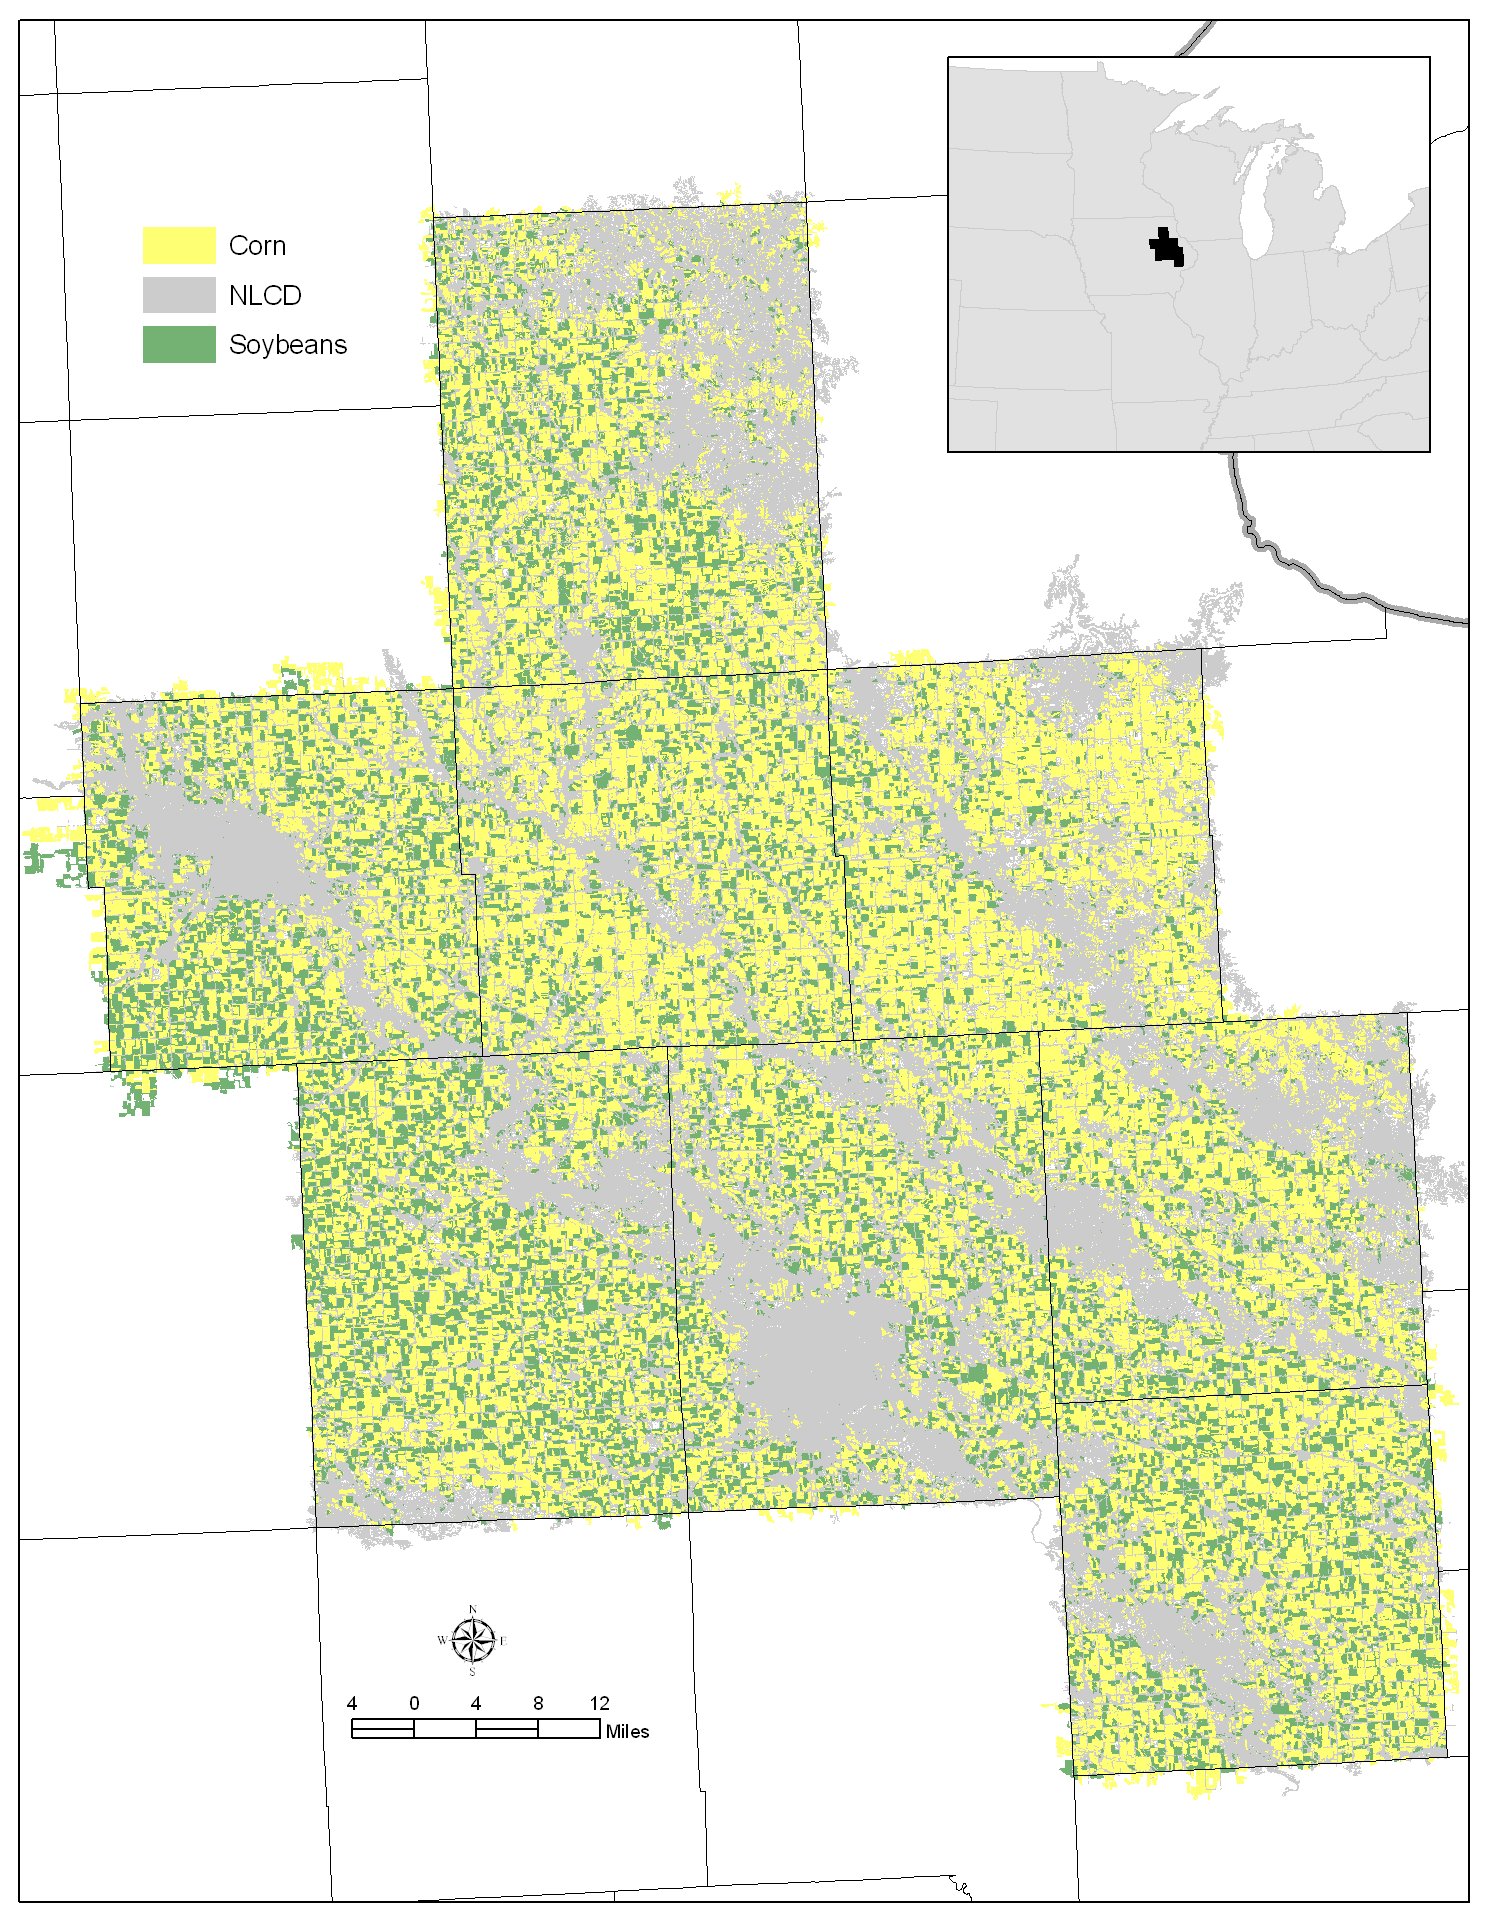
\includegraphics[width=0.45\textwidth]{iowa/crops_iowa.png}  
  }
  \subfigure[SSURGO Soils]{
    \label{fig:soil}
    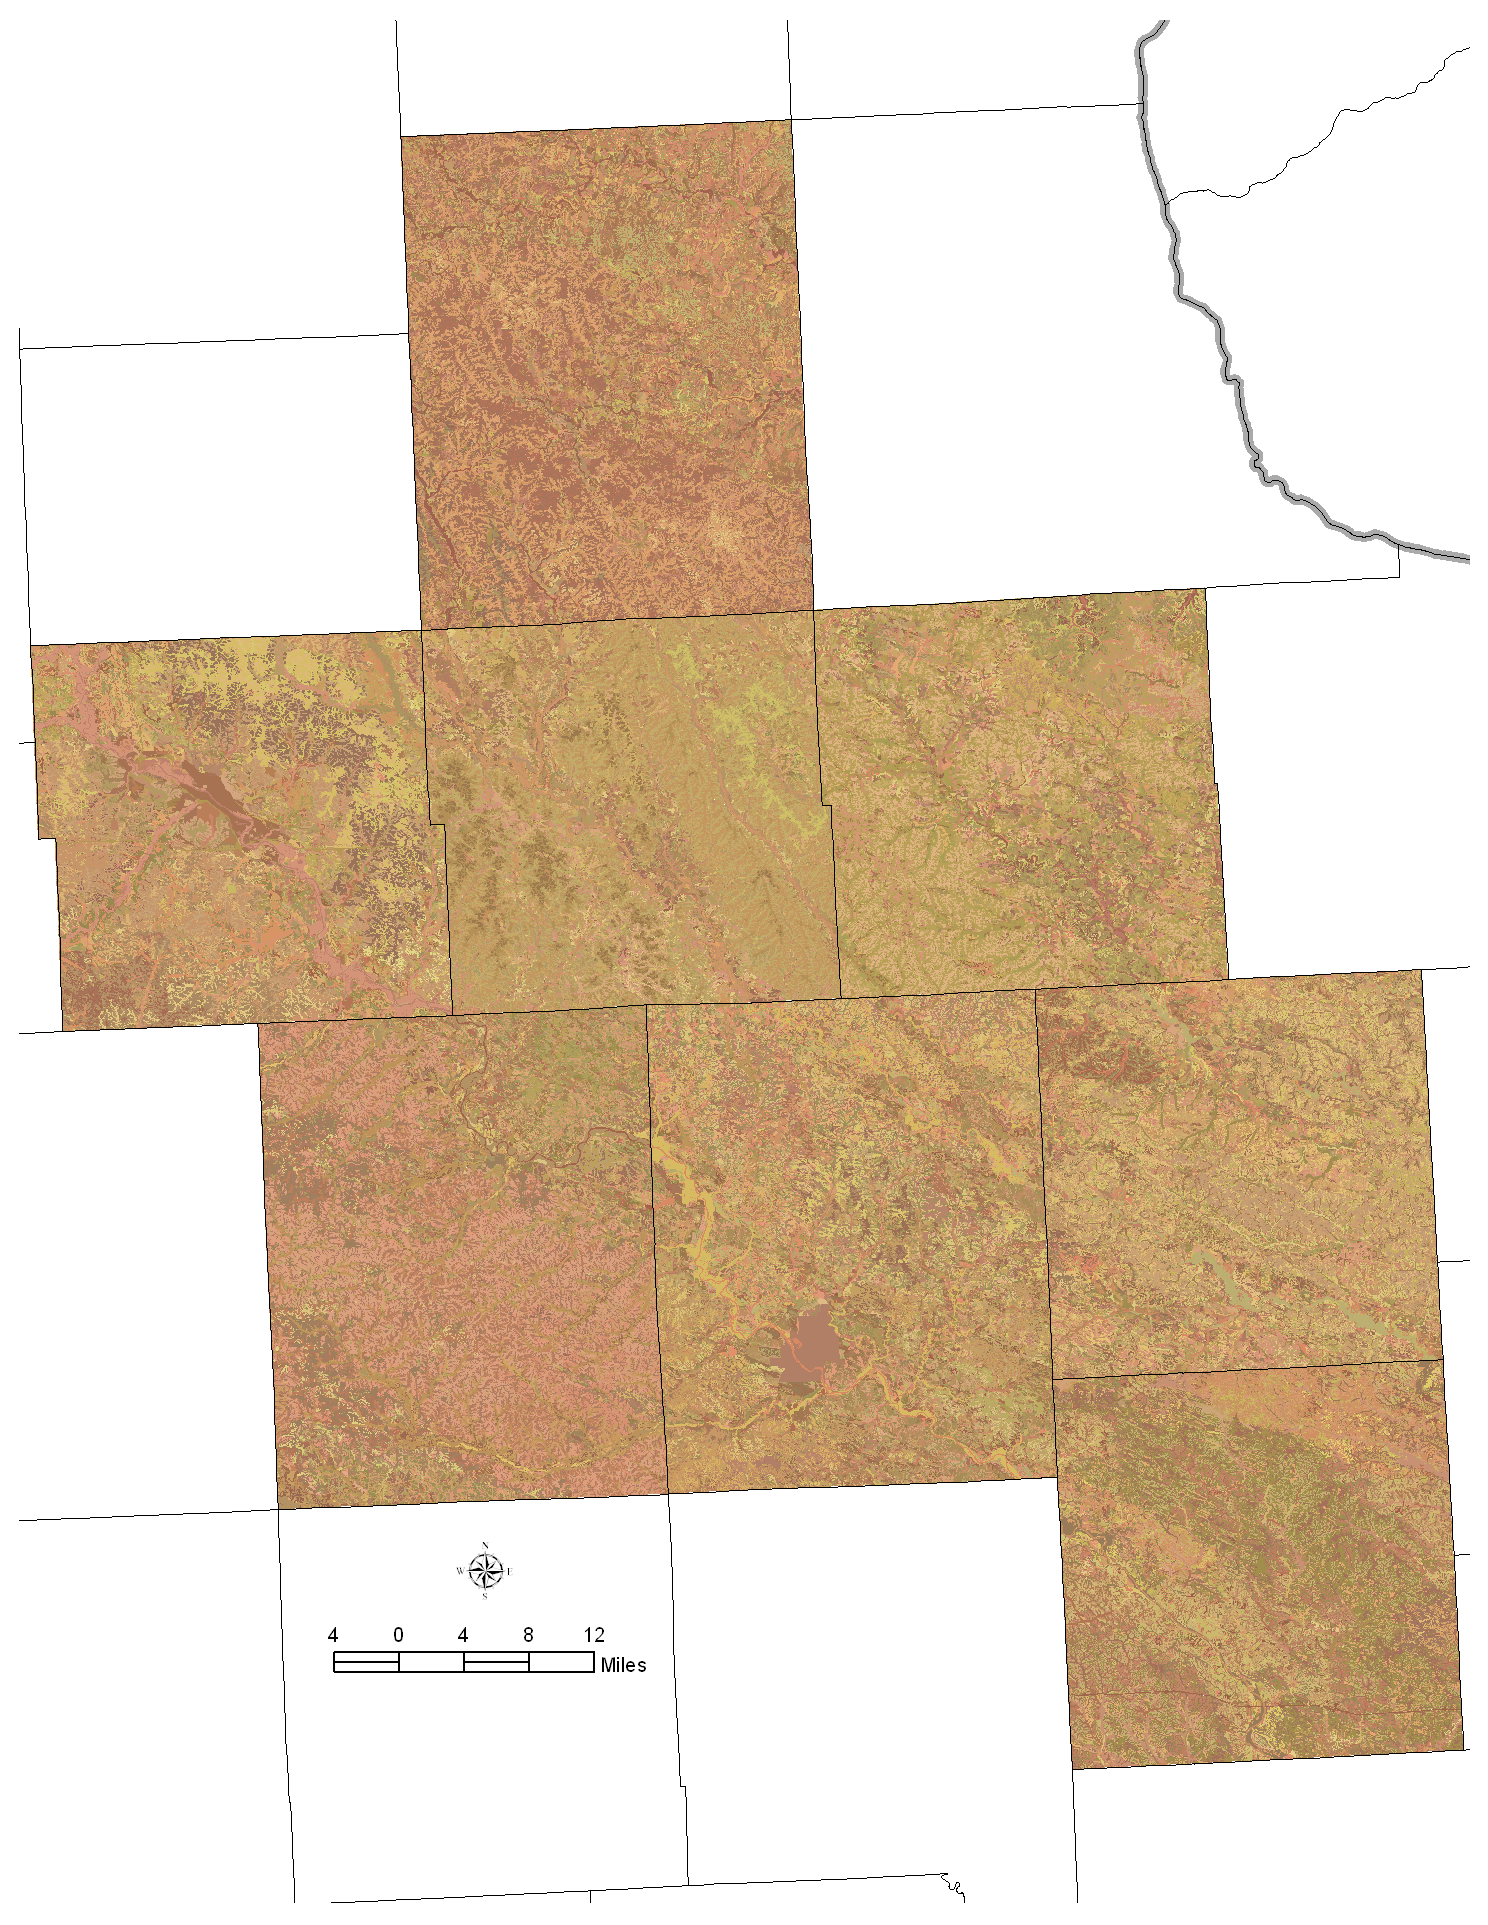
\includegraphics[width=0.45\textwidth]{iowa/ssurgo_iowa.png}  
  }
  \caption{Corn study Area}
  \label{fig:study-area}  
\end{figure} Wheat straw production is addressed in a X county region of Kansas. Forest residues are addressed in northern California (figure XXX). To conduct the analysis we use a base case consisting of feedstock supply aggregated to the county from \ac{NASS} agricultural production data or in the case of forest residue from the \ac{FPL}. Supply curves are calculated for delivered biomass to potential biorefineries in the region. Harvest costs are calculated based upon standard machinery configuration for a each feedstock type. Transport costs are calculated using least-cost routing from the point of origin to potential facility location.  We compare the base case with a high-resolution feedstock model which locates the feedstocks to a geographic area representative of the size of an operational unit (farm or forest harvest unit). Harvest and transport costs are calculated similarly in the high-resolution model though in the high resolution model, each operational unit is located on the transportation network so that the intra-county cost calculation is eliminated.

\subsection{Base case}

In the base case we use feedstock production aggregated to the county level. We create coordinate point locations at the centroid of each county within the study region. The point location represents the supply of each distinct feedstock across a range of prices. To estimate the intra-county transport cost we use a county level data is aggregated to a point at the geograpic centroid of the county. This cost is calculated using the average “city-block” distance from any point in the county to the centroid.  This geometric measure uses the perimeter of the county to estimate average travel distance (average distance is approximately $P_s/8$ where $P_s$ is the perimeter of the service area or county).  Additionally, it is assumed that the average travel speed along this route is 35 mph.  These intra-county costs are then combined with the county centroid-based network transportation model.

\subsubsection{Feedstock mapping}
Corn and wheat production by county is extracted from NASS......

\subsubsection{Harvest cost}
 The \ac{INL} has developed an economic model for the delivery of agricultural residues from the field to the biofuel processing plans. The model derives costs for in-field activities as well as loading and transport costs from field to biorefinery.  The model calculates delivered feedstock costs based upon a single feedstock species, supply chain configuration, and user defined  transport distance.
\subsubsection{Transport cost}
Biomass transportation costs were modeled using three modes: truck, rail, and barge.  Figure \ref{fig:centca_network} shows an example of this network. Trucking costs have three components: a loading/unloading cost, a time-dependent travel cost, and a distance-dependent travel cost.  The time and distance dependence allow for differential cost between traveling on slow local roads versus fast interstate highways.  

The costs of biomass transport by road, rail  and marine are described in Table~\ref{transcost}.  Trucking costs \citep{Jenkins2000,Perlack2003,Reynolds2002} do not vary by feedstock type and depend only on truck payload. Network trucking costs are calculated from the cost/ton-mile and distance traveled. Biomass transportation costs are assumed to be on a wet basis.  Diesel fuel cost is assumed to be  \$2.50 per gallon.  Rail costs are calculated from a  mileage-based rate schedule for agricultural products \citep{Railroad2007}. 

Marine transportation costs are based on a published rate schedule for inland barge transport \citep{Tidewater2007}.  The rates were fitted to a linear function of distance similar to the rail rates above. 
\begin{table}[h]
\centering
\begin{tabular}{c p{3cm} c c} 
\textbf{Mode}& \textbf{Cost component}  & \textbf{Bulk solids} \\ \hline \hline
road& Loading/ unloading  & $\$5\cdot \text{wet ton}^{-1}$   \\ 
road& Time dependent  & $\$29\cdot \text{hr}^{-1}/ \text{truckload}$  \\ 
road& Distance dependent  & $\$1.20\cdot \text{mile}^{-1}/ \text{truckload}$ \\ 
road& Truck capacity  & 25 wet tons \\ \hline
rail& Loading/unloading  & $\$5\cdot \text{wet ton}^{-1}$ \\ 
rail& Fixed Cost &  $\$27\cdot \text{wet ton}^{-1}$ \\ 
rail& Distance dependent  & $\$0.023\cdot \text{mile}^{-1}/\text{wet ton}$ \\ 
rail& Rail Car Capacity  & 106.5 wet tons \\ \hline
marine& Loading/unloading  & $\$5\cdot \text{wet ton}^{-1}$ \\ 
marine& Fixed Cost  & $\$3.85\cdot \text{wet ton}^{-1}$ \\ 
marine& Distance dependent  & $\$0.043\cdot \text{mile}^{-1}/\text{wet ton}$ \\ 
marine& Barge Capacity  & 4,000 wet tons \\\hline
\end{tabular}
\caption{Transportation cost factors. Time dependent road costs include labor and capital. Distance dependent road costs include fuel, insurance and maintenance.}
\label{transcost}
\end{table}


\subsection{Hi-resolution case}

In the high resolution case we dis-aggregate county level supply estimates to areas representative of individual farms within the county. Figure~\ref{fig:overview} shows a basic overview for determining the variation on harvest yield for an agricultural region.  The process involves dividing the region in to  a regular grid of \emph{pseudo-farms} of a size representative of the average farm size in the county, deciding which of these farms are in production of the target crop based on a satellite image derived crop type map, establishing suitability of the soil at each \emph{pseudo-farm}, and then assigning yields to \emph{pseudo-farms} based on the county estimates.

\begin{figure}[hpt]
  \centering
  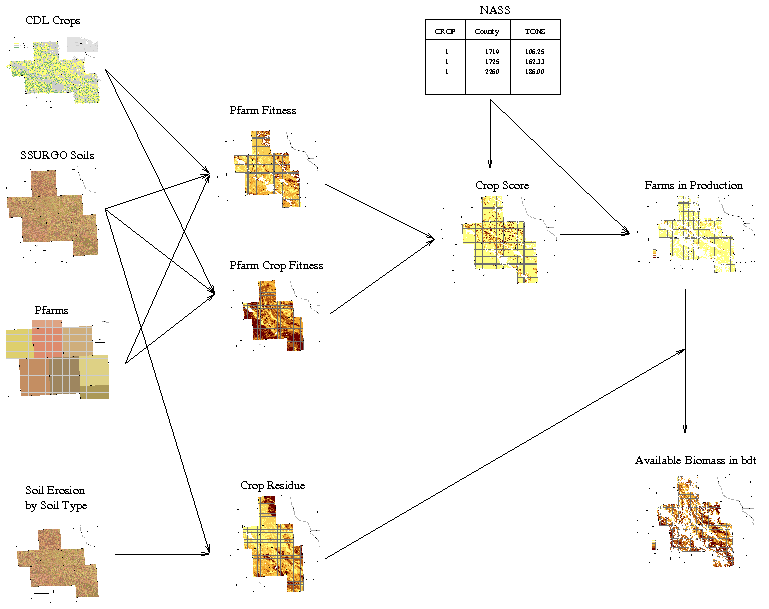
\includegraphics[width=0.75\textwidth]{iowa/maps.png}  
  \caption{Overview}
  \label{fig:overview}
\end{figure}

\subsubsection{Pseudo-farms}

First, the region is divided into a series of \emph{pseudo-farms} (Figure~\ref{fig:pfarms}). For each pseudo-farm, a number of fitness variables are assigned to model where crops will be grown, and their yields.

\emph{Farm fitness}~(Figure~\ref{fig:fitness}), is a score without a specific crop assigned to pseudo farm which gives the total amount of arable land and the average land capability.  Farms need to be more then 10\% arable to be included, otherwise it is considered not farmed.

For a specific crop, \emph{Pseudo-farm crop fitness}~(Figure~\ref{fig:crop-fitness}), represents the amount of area either identified as that crop within the \emph{pseudo-farm} , or identified as typical crop for the underlying soil types.  Also this fitness value includes expected yield for specific crops.
The \emph{Farm crop score} combines NASS cropland types and SSURGO
fitness, for the crop and in general.  Areas with both get scored
highest.


\begin{figure}[hpt]
  \centering
  \subfigure[Pseudo-farms]{
    \label{fig:pfarms}
    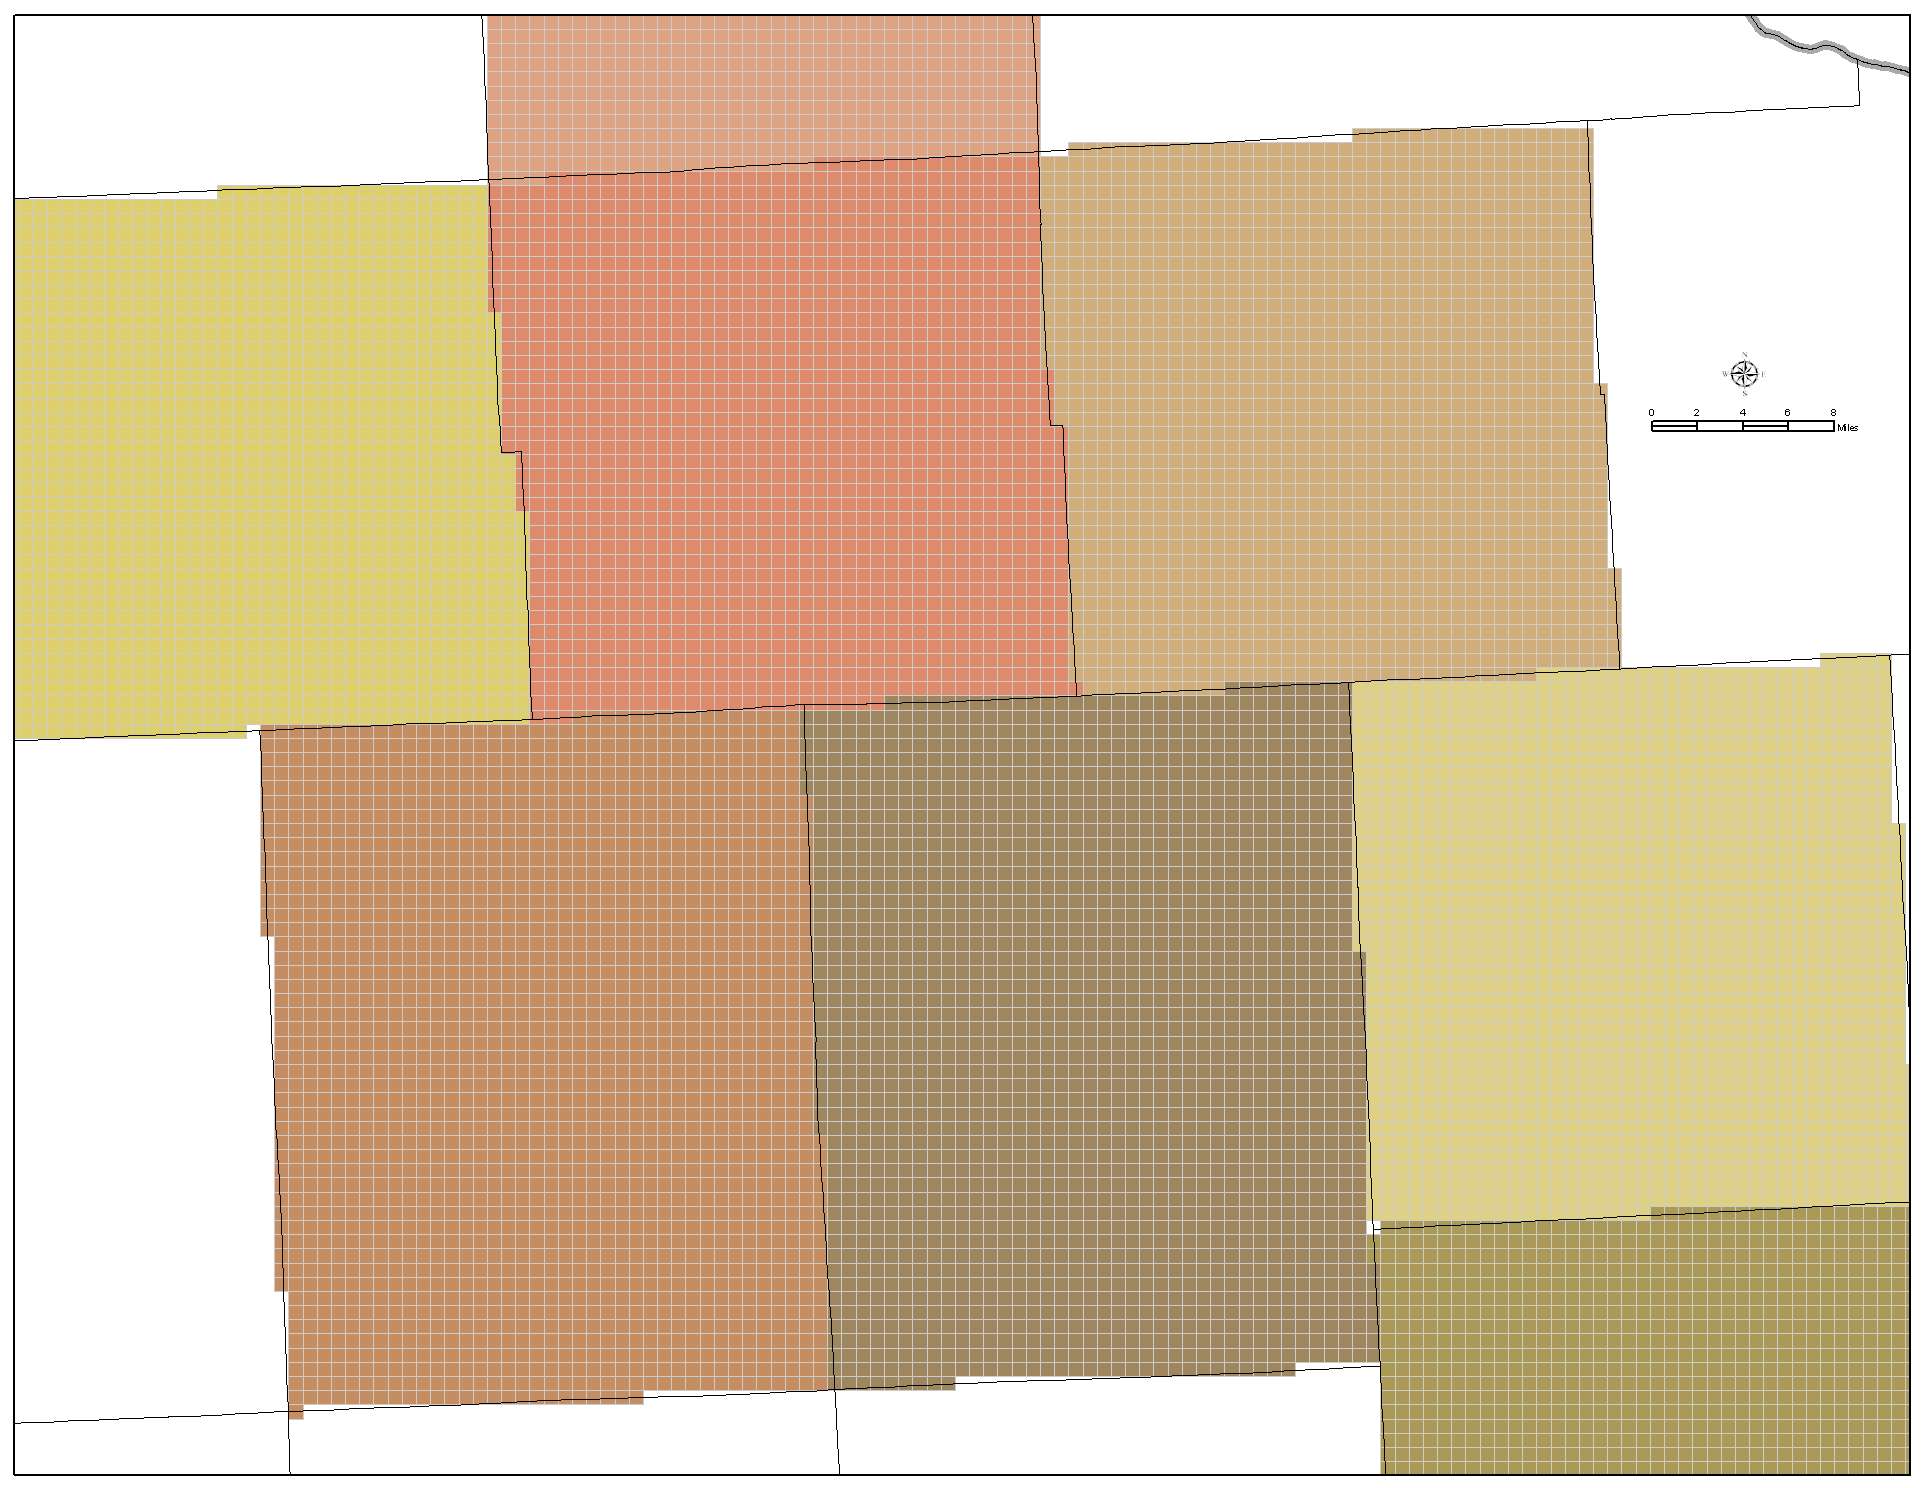
\includegraphics[width=0.45\textwidth]{iowa/pfarms.png}
  }
  \subfigure[Pseudo-farm fitness] {
    \label{fig:fitness}
    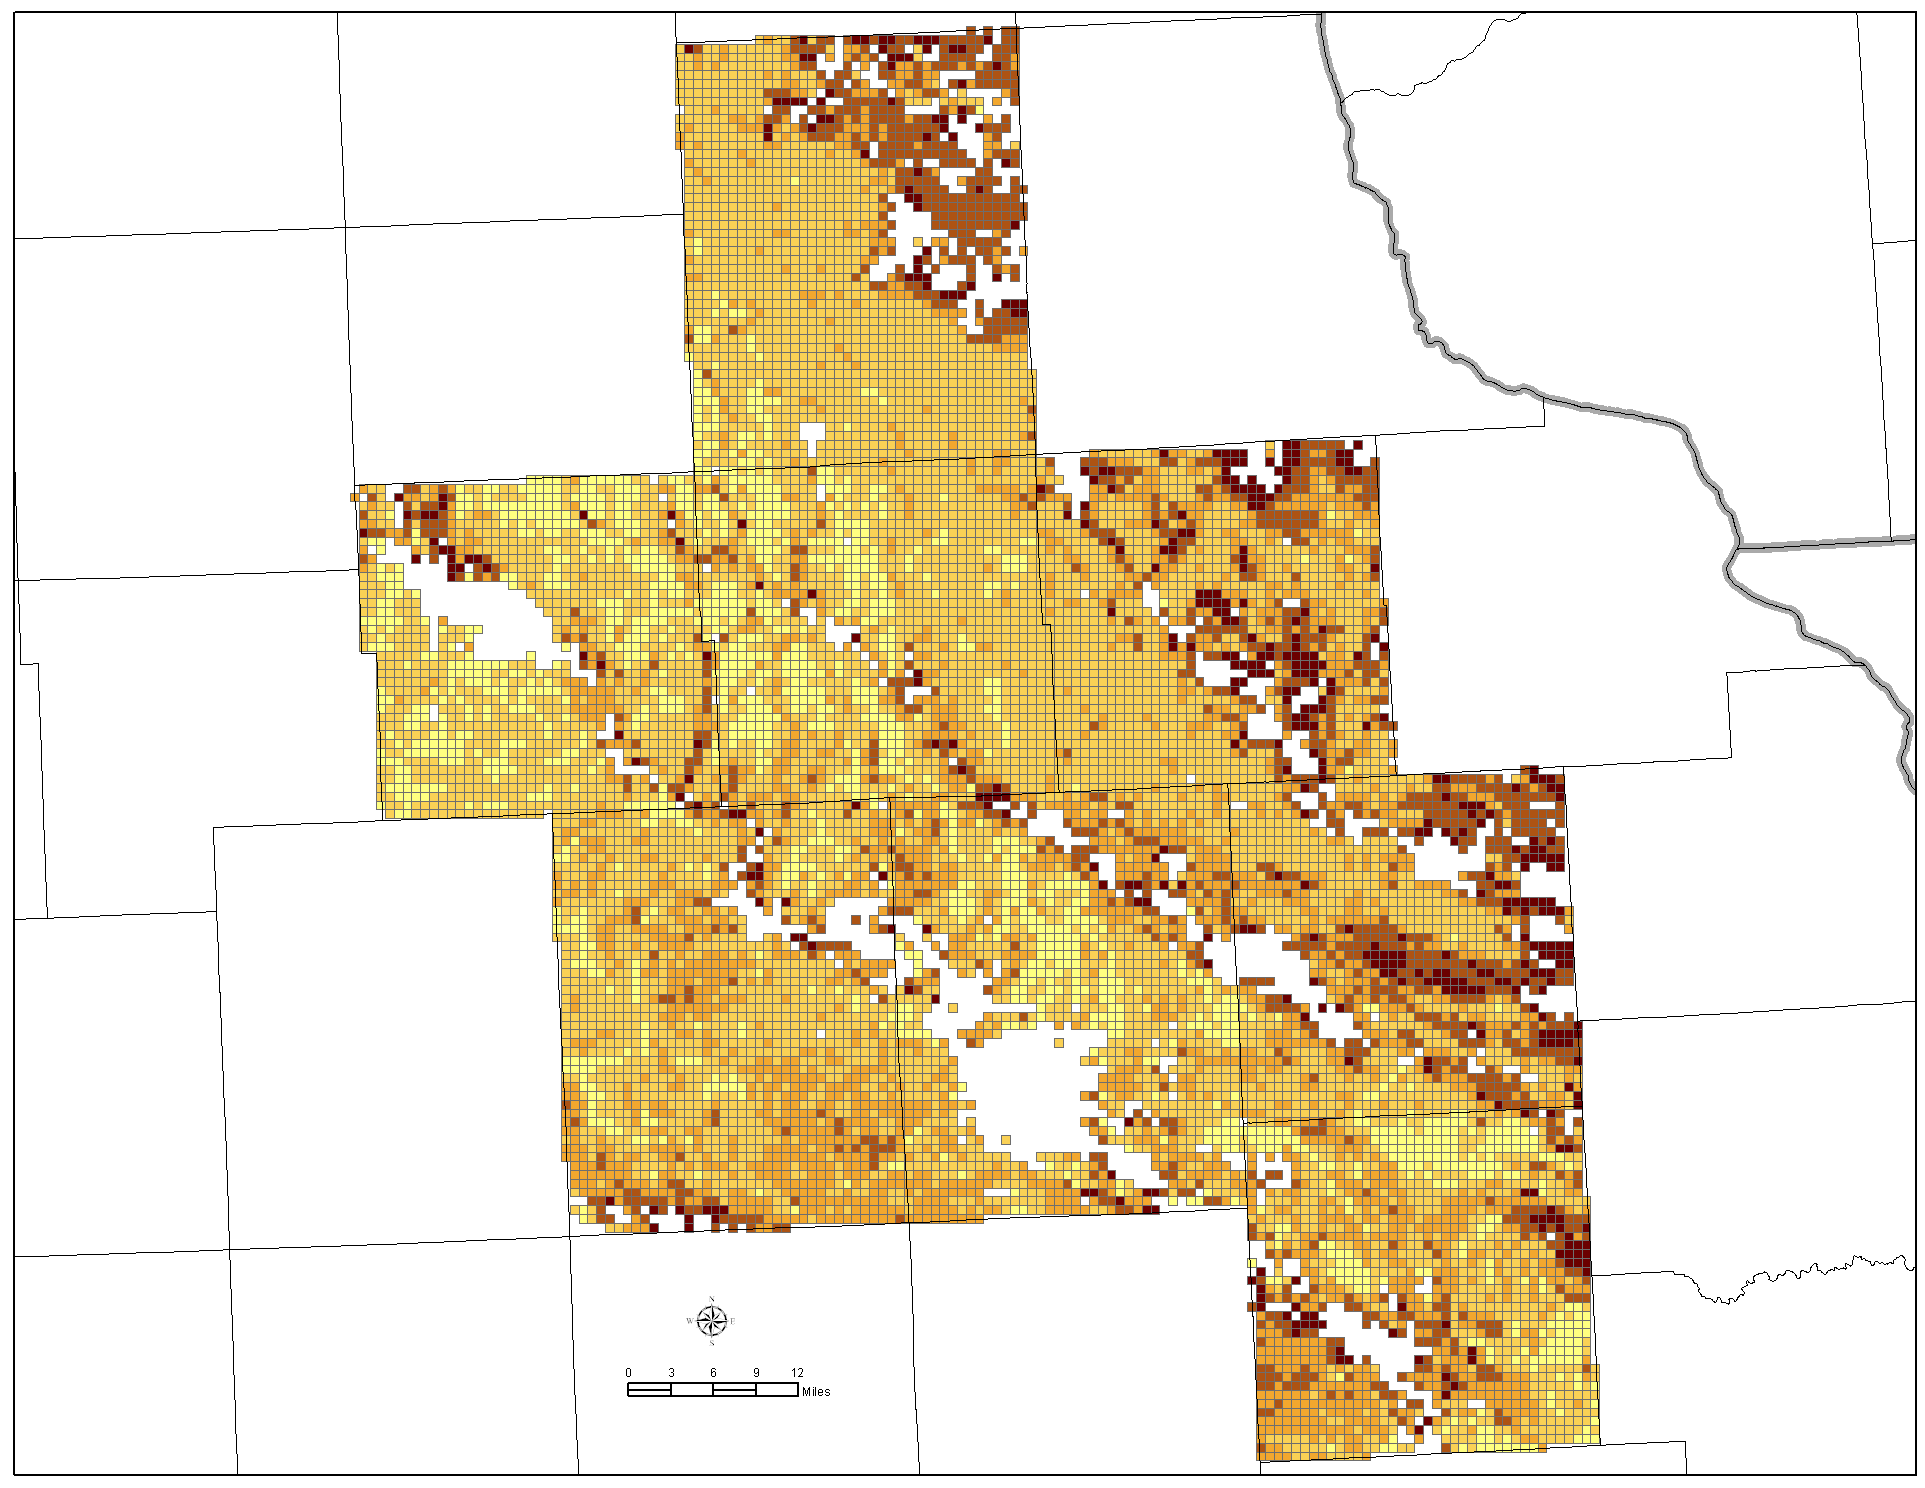
\includegraphics[width=0.45\textwidth]{iowa/pfarms_fitness.png}  
  }

  \subfigure[Pseudo-farm crop fitness]{
    \label{fig:crop-fitness}
    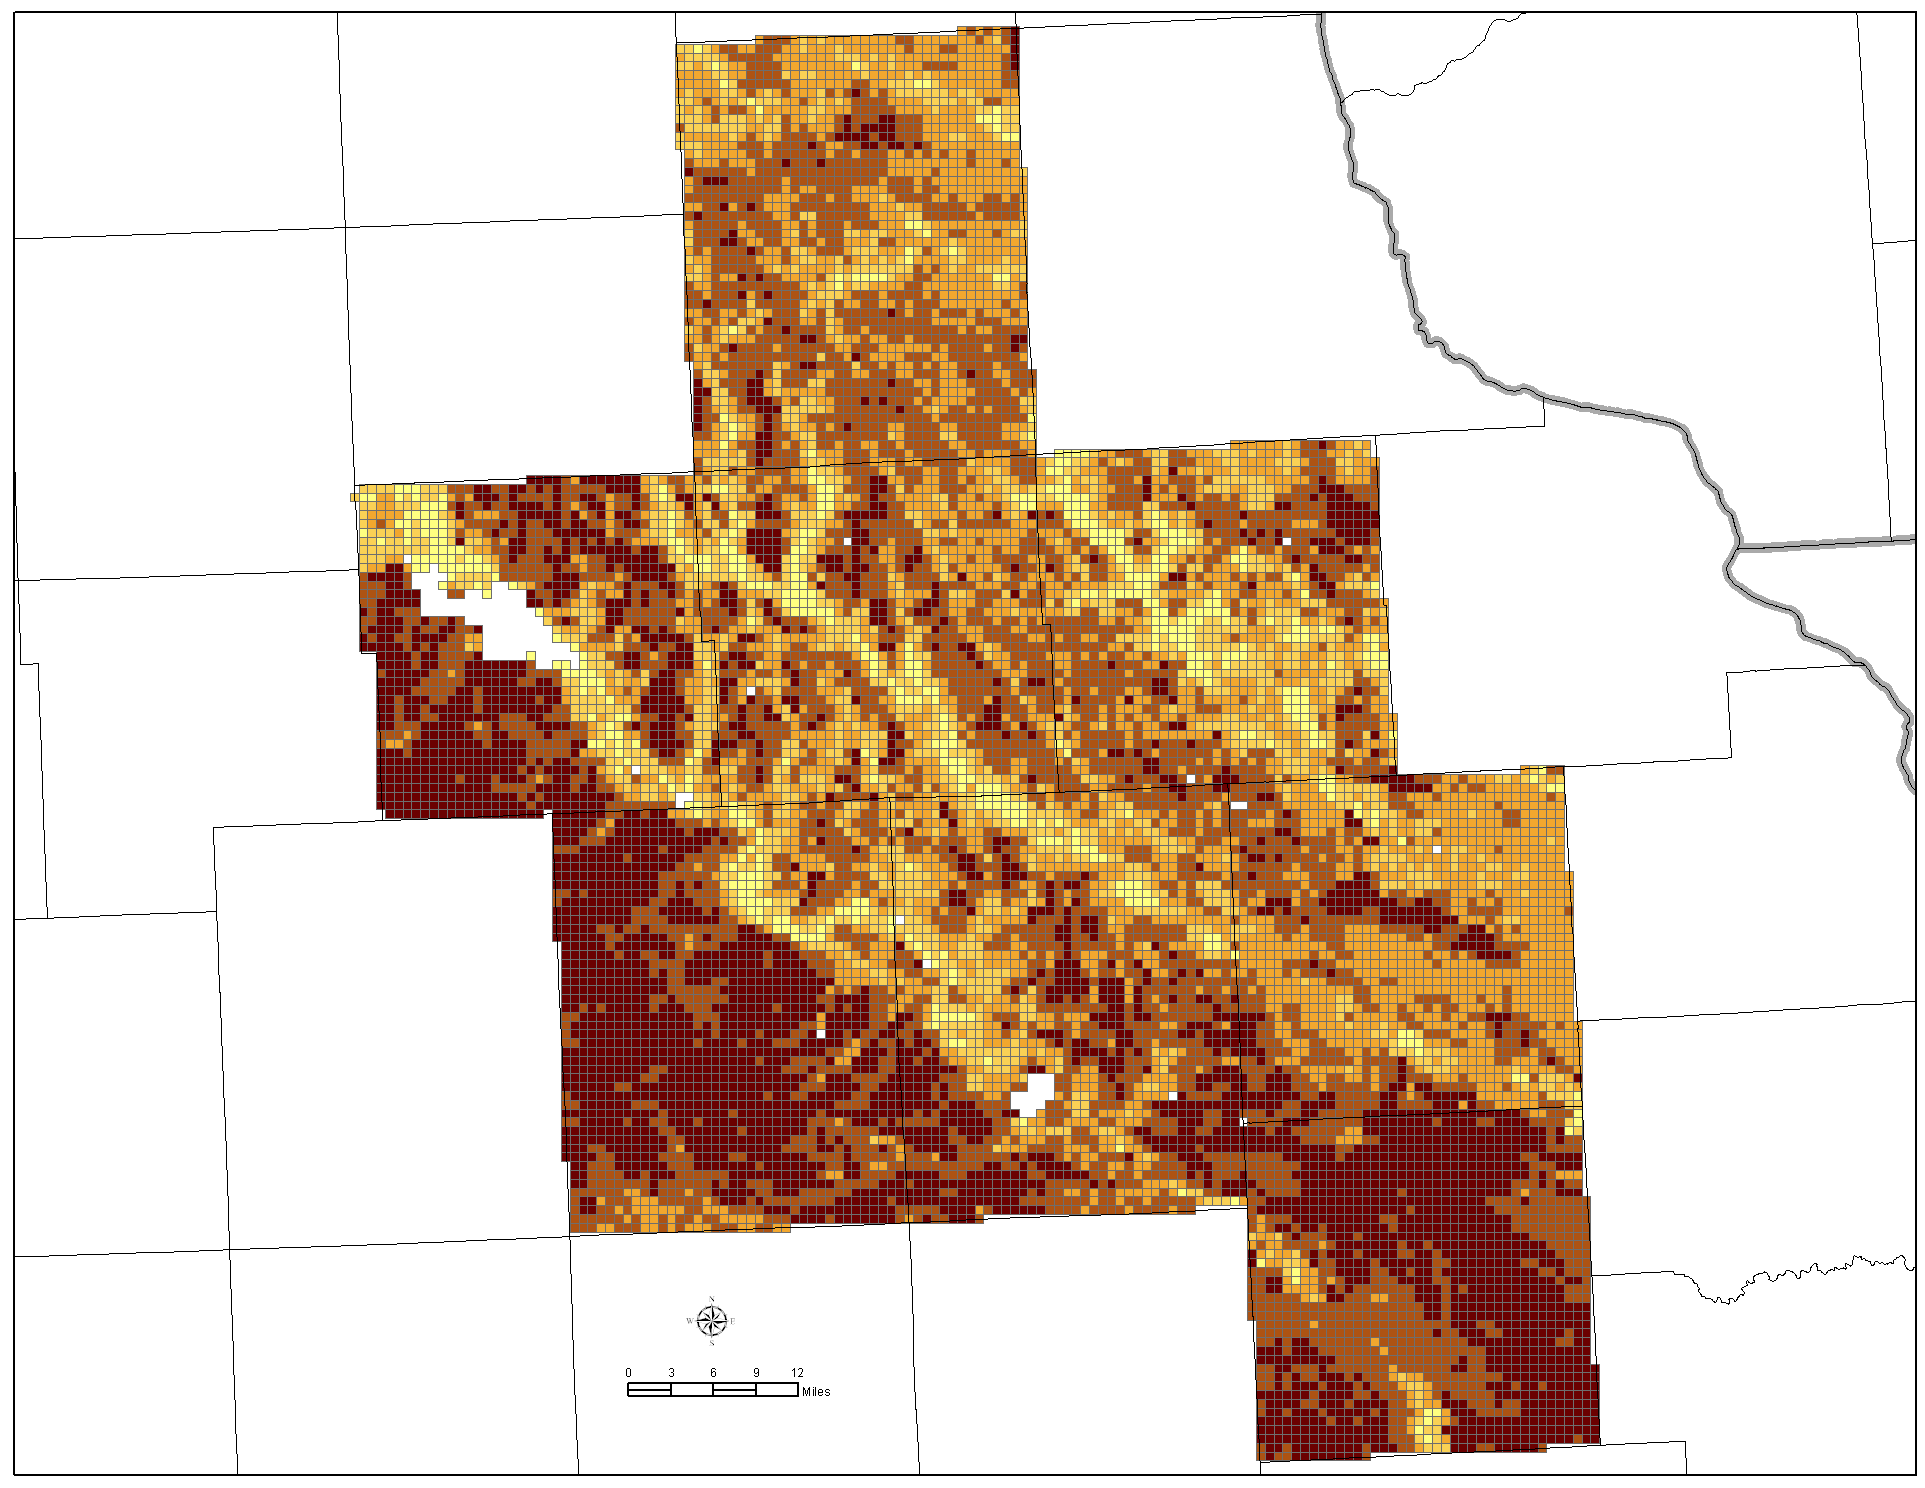
\includegraphics[width=0.45\textwidth]{iowa/pfarms_crop_fitness.png}  
  }
  \subfigure[Pseudo-farms Score] {
    \label{fig:scoring}
    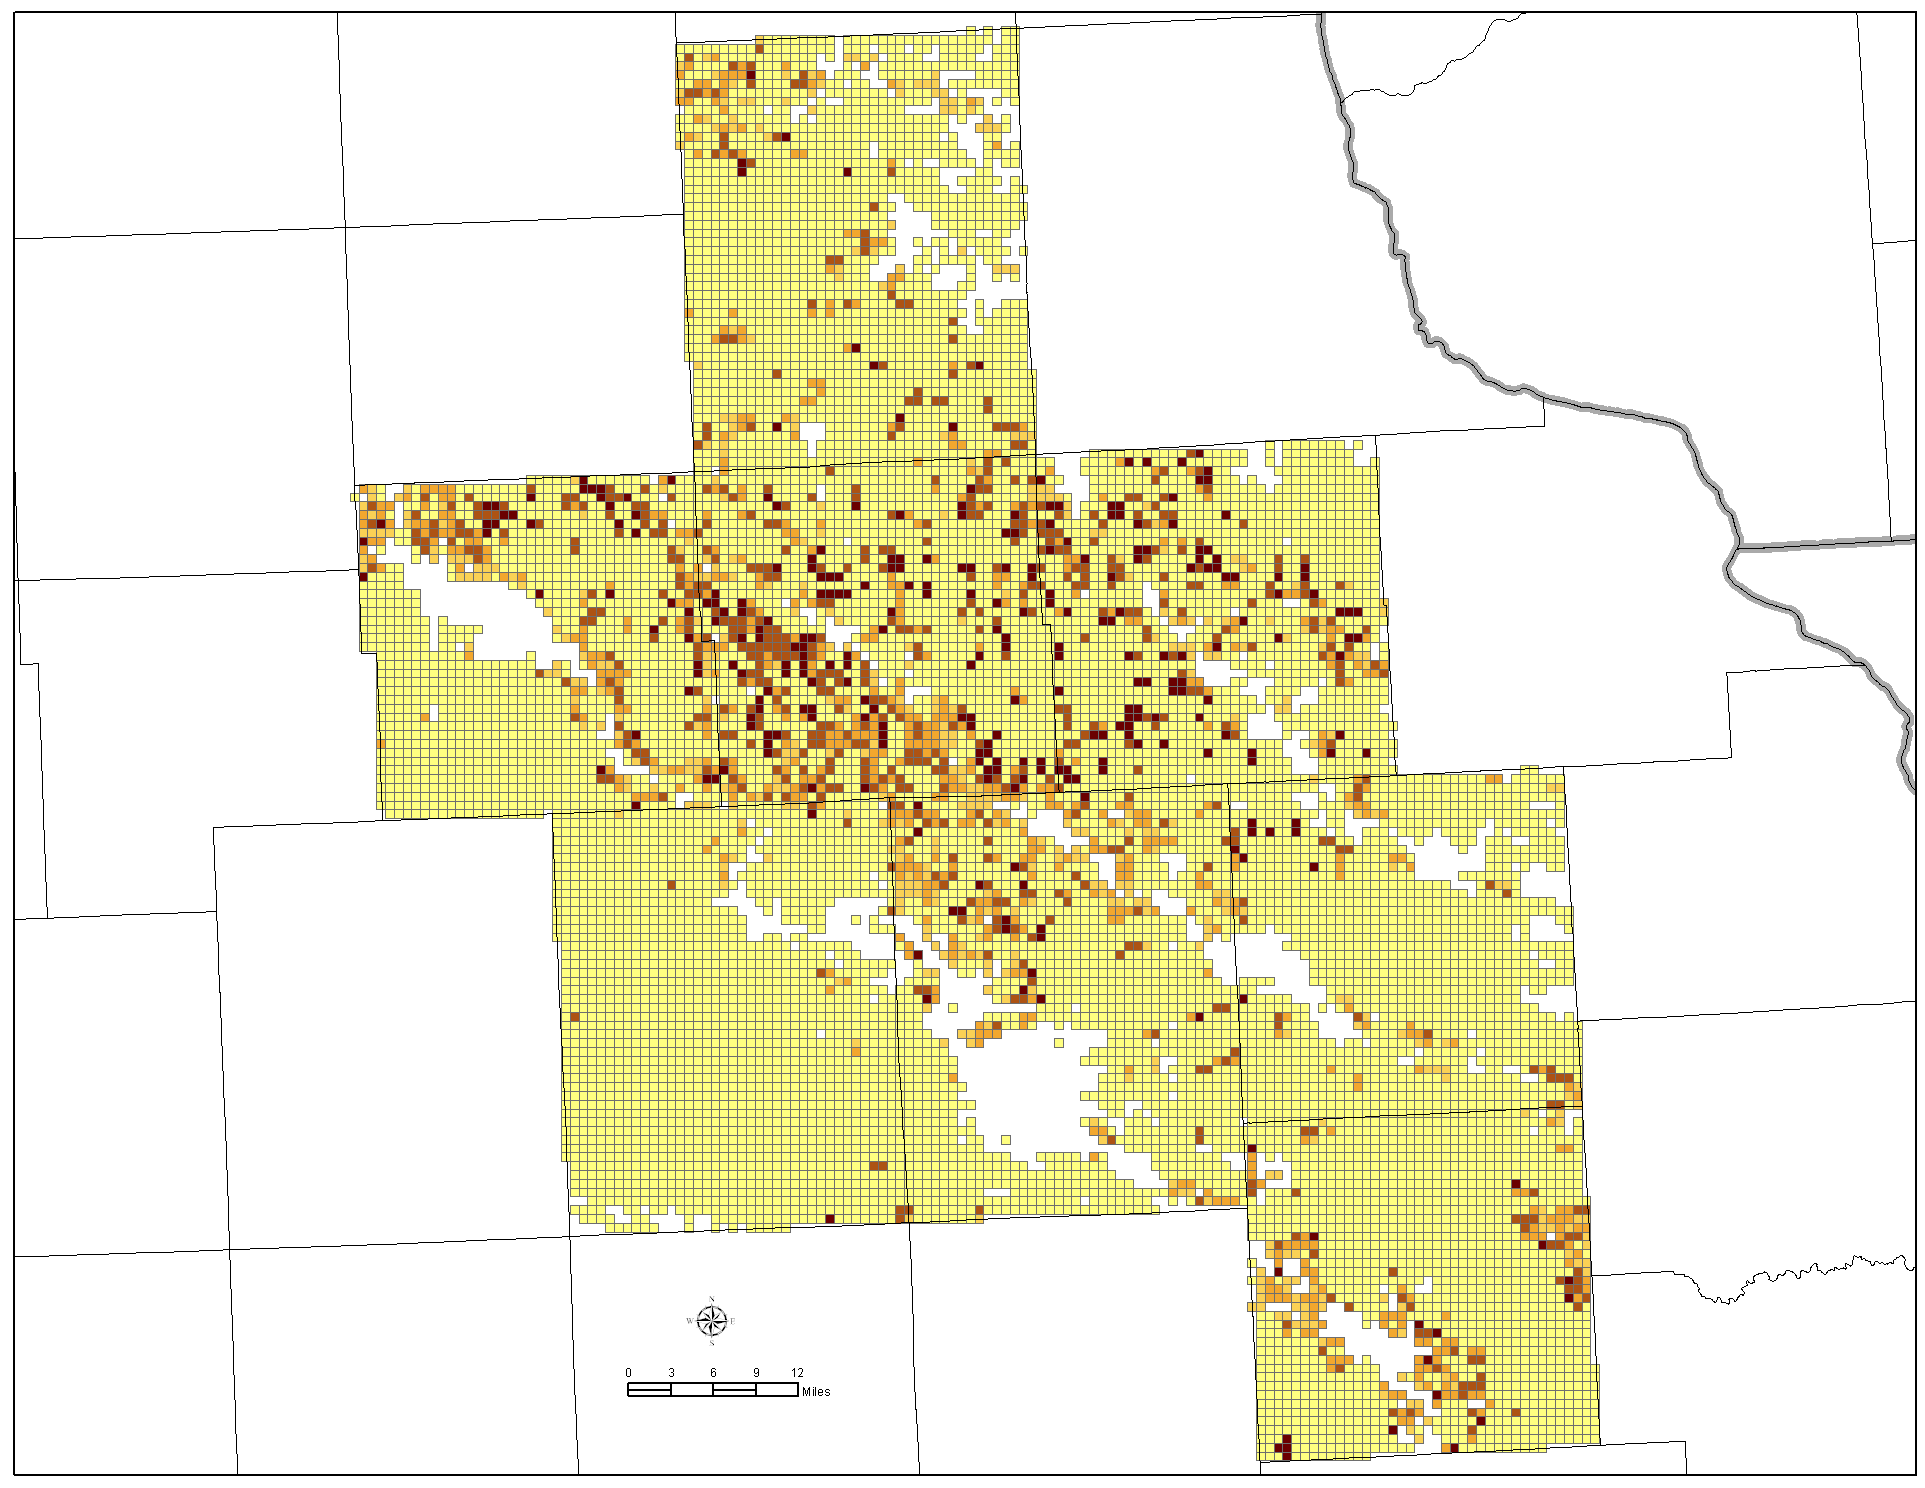
\includegraphics[width=0.45\textwidth]{iowa/pfarms_crop_score.png}  
  }
  \label{fig:scores}
  \caption{Pseudo-farm scoring}
\end{figure}


For a particular crop type and expected acres harvested the most
likely pseudo-farms to be planted are selected. Actual, per-county
production amounts are used to establish pseudo-farms in production for a
specific year.  Once the farms are selected, we adjust the yields
within the farms to match the total county output. Use an average
yield for soils without crop yields (Figure~\ref{fig:actual}.

Once yields are calculated, the amount of biomass recovered needs to
be determined. Each pseudo-farm has a soil type and slope that affects
how much residue needs to be left on for tolerable soil
loss~(Figure~\ref{fig:biomass}).

Use the bushels of predicted corn to estimate the standing biomass,
and remove the residue needed, to produce a map of standing biomass
per pseudo-farm~(Figure~\ref{fig:actual-bio}).


\begin{figure}[hpt]
  \centering
  \subfigure[Pseudo-farms in Actual Production]{
    \label{fig:actual}
    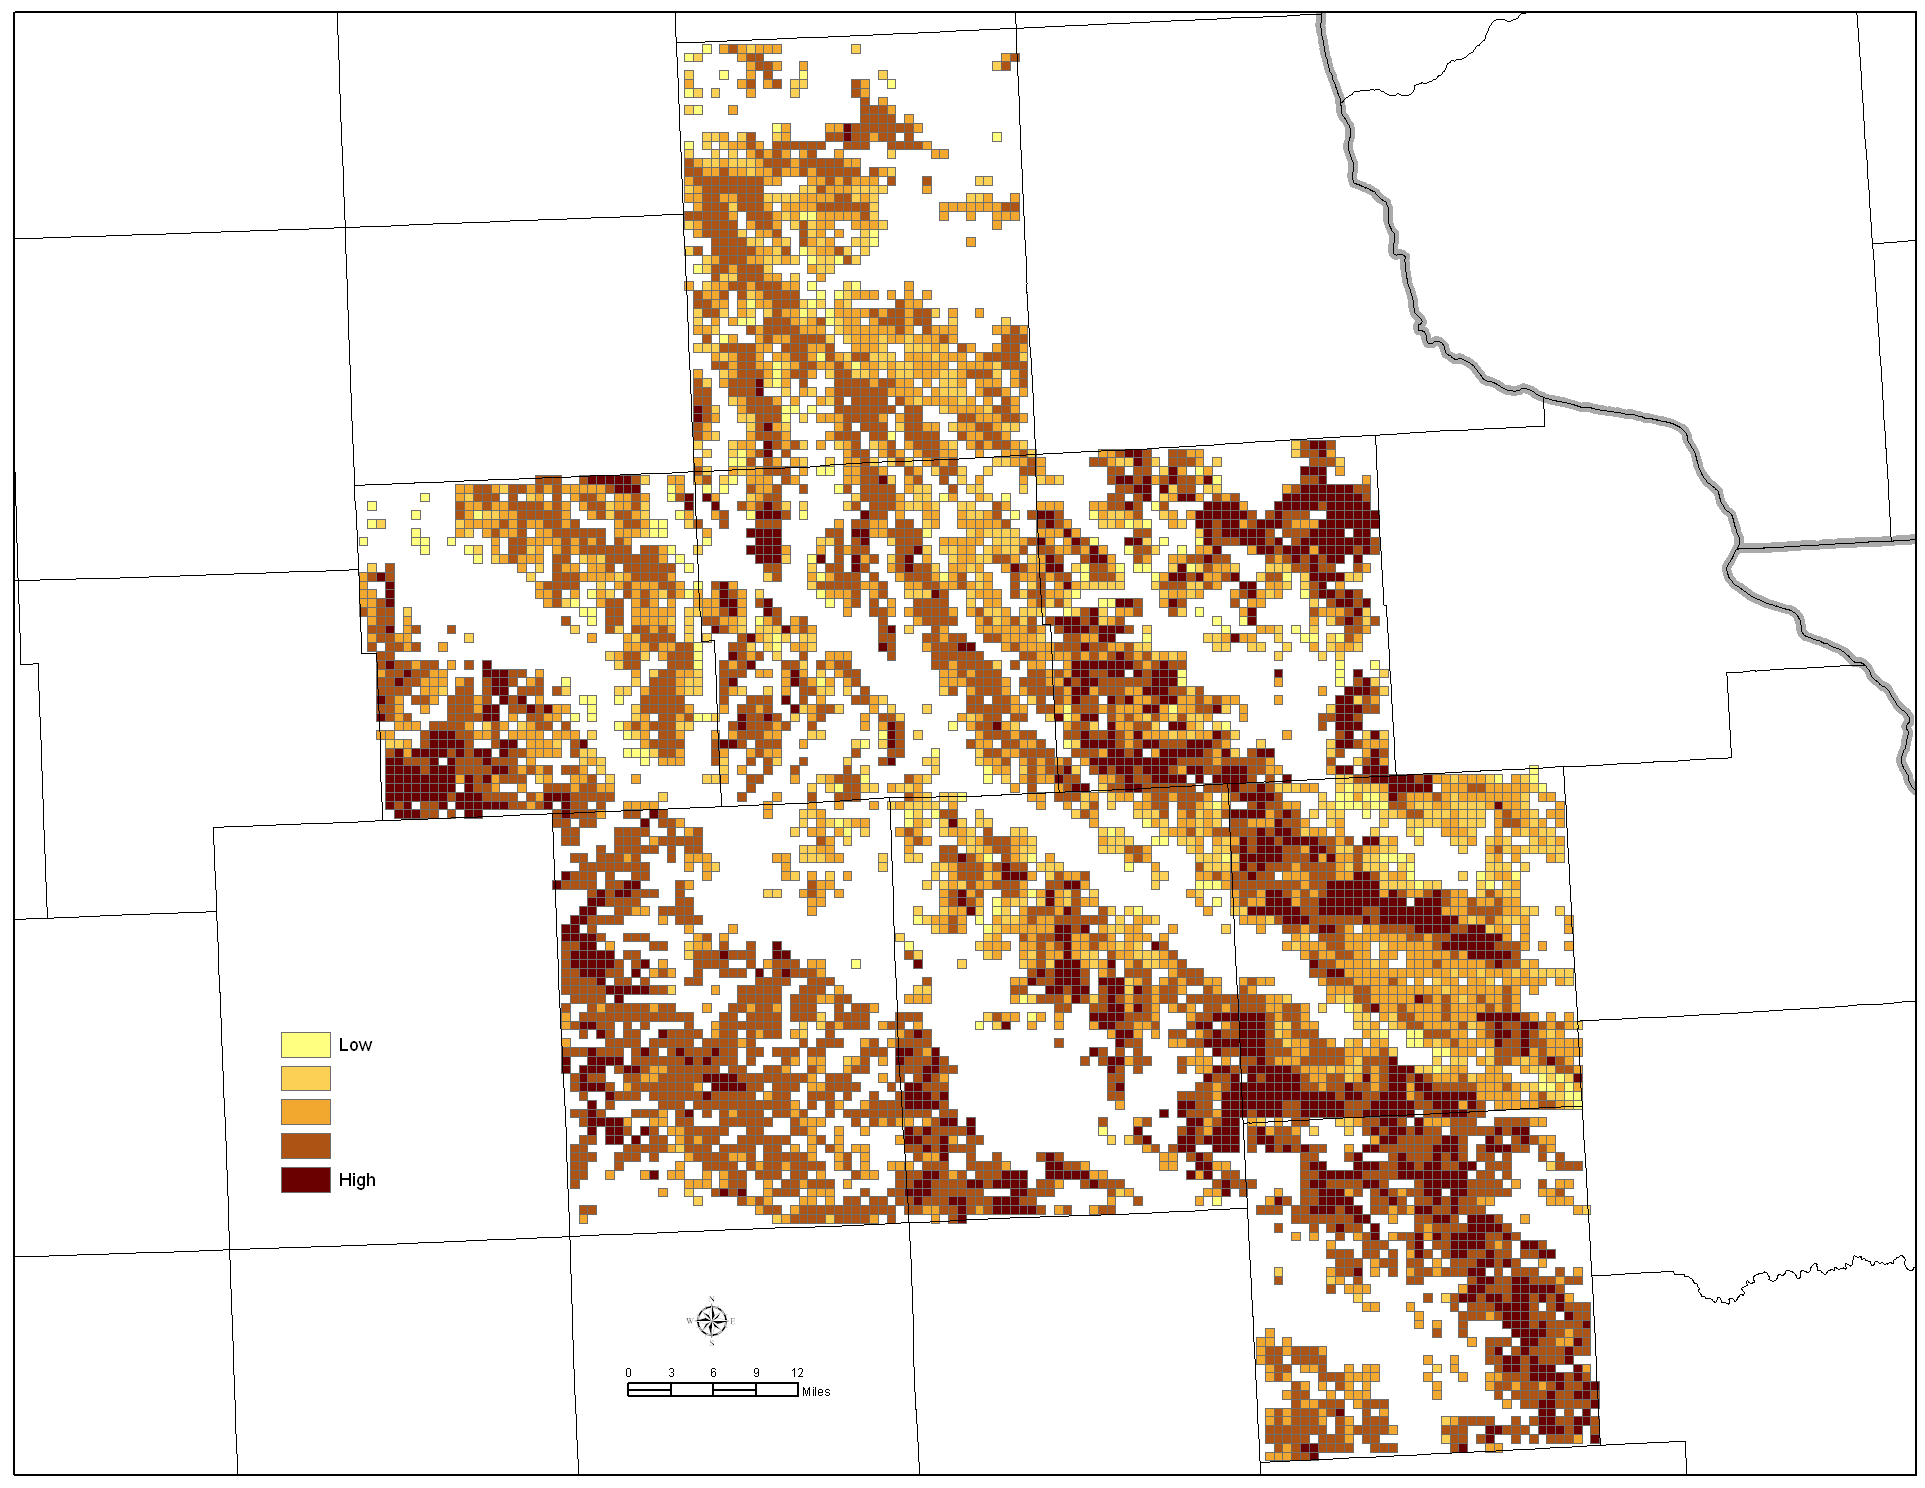
\includegraphics[width=0.45\textwidth]{iowa/m_pfarms_actual_production.png} 
  }
  \subfigure[Crop residues] {
    \label{fig:biomass}
    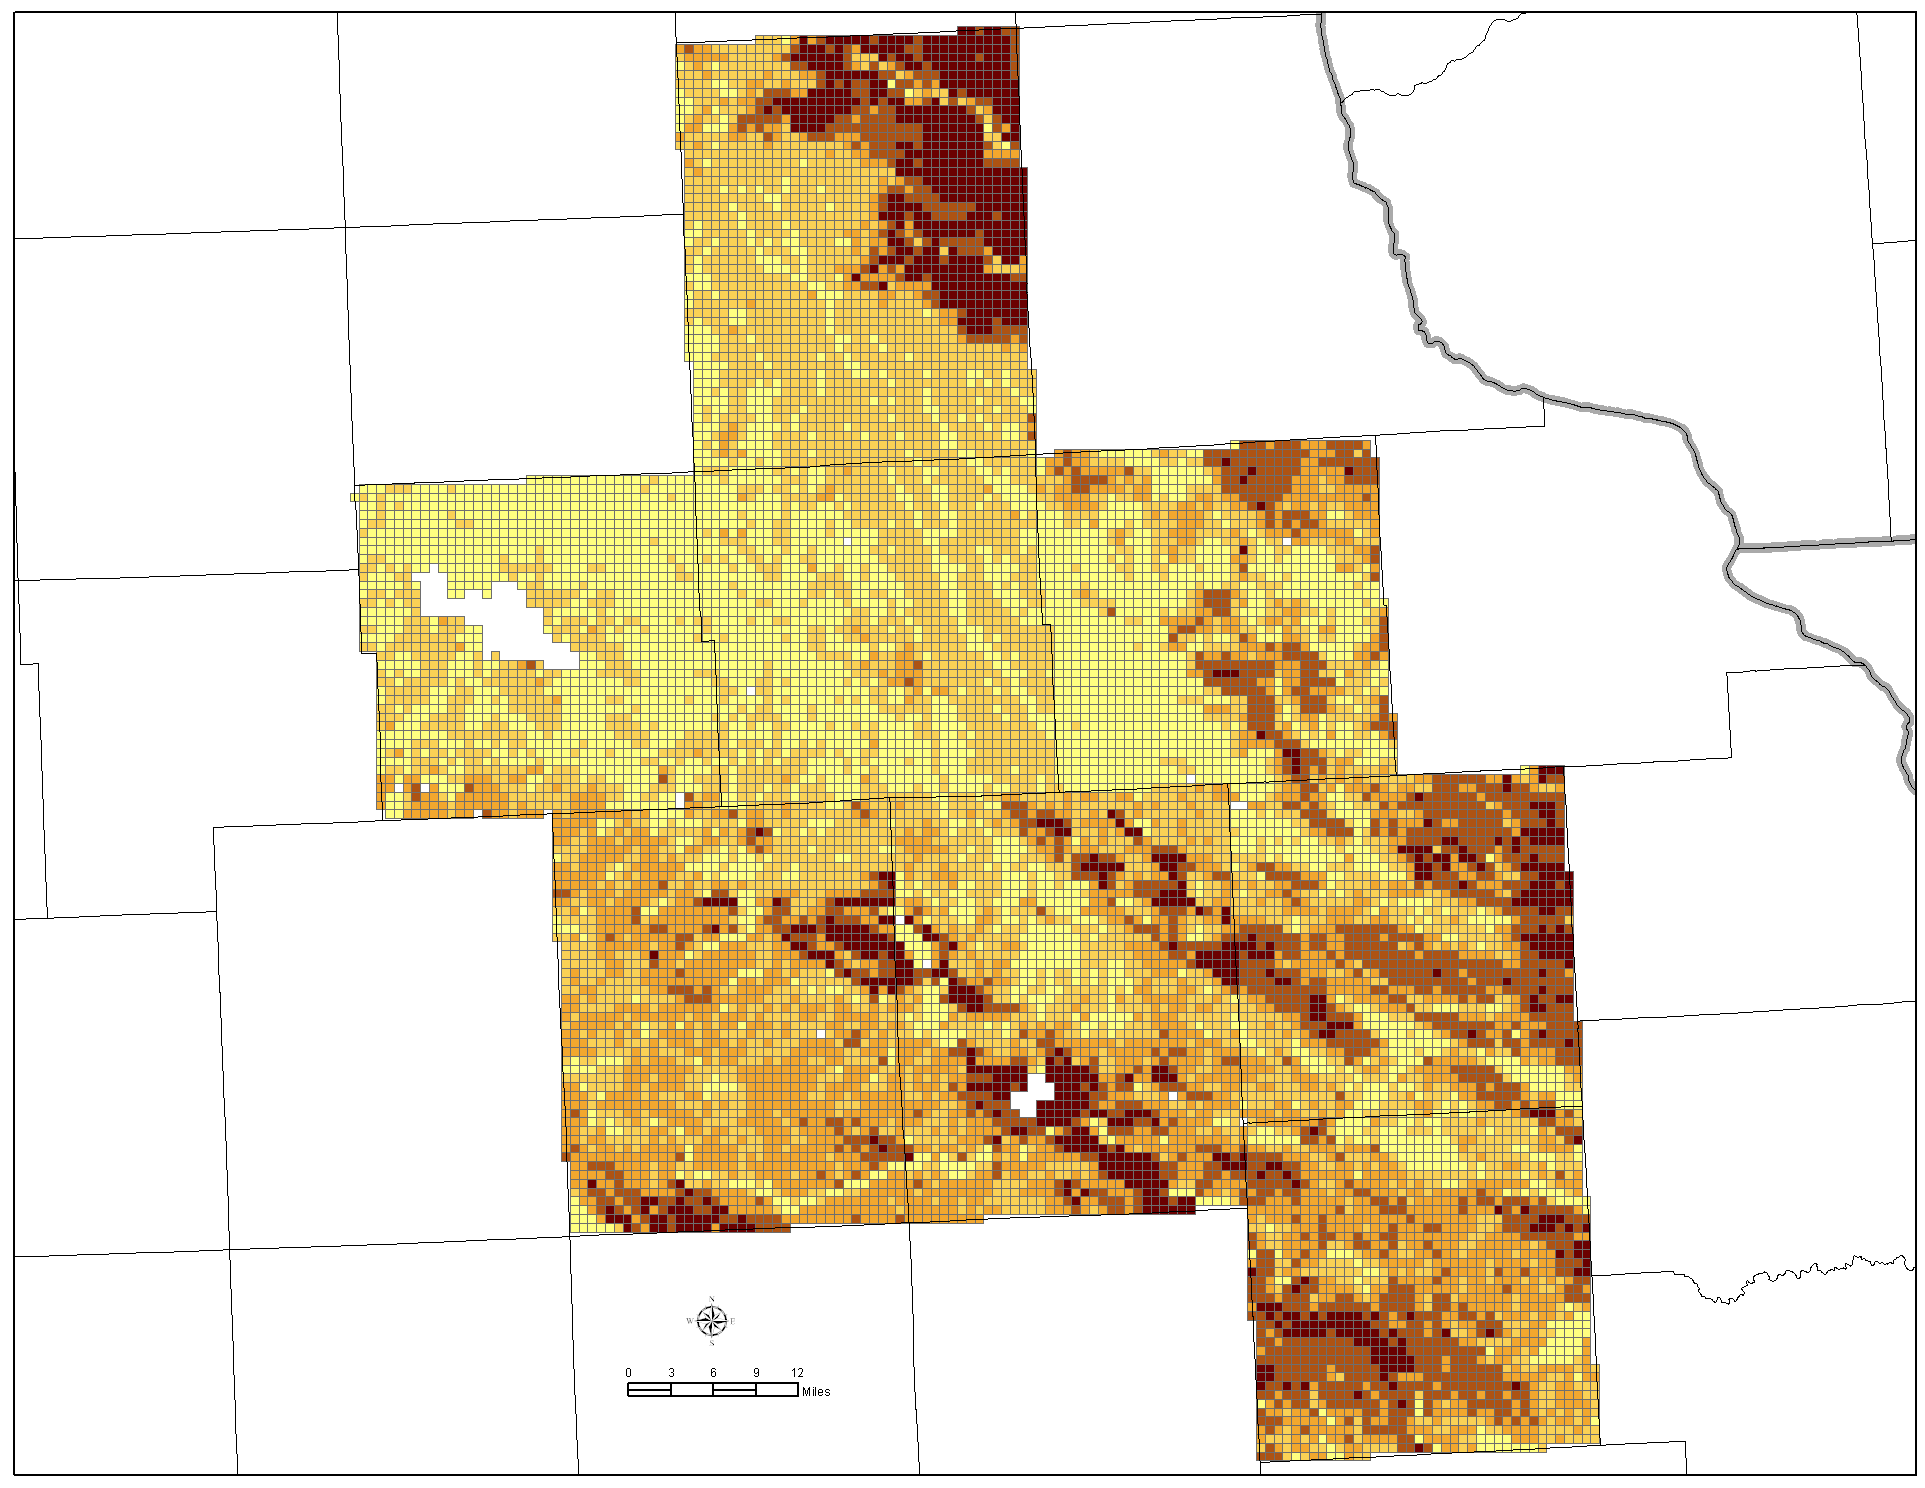
\includegraphics[width=0.45\textwidth]{iowa/pfarms_crop_residue.png}  
  }
  \subfigure[Pseudo-farm yields] {
    \label{fig:actual-bio}
    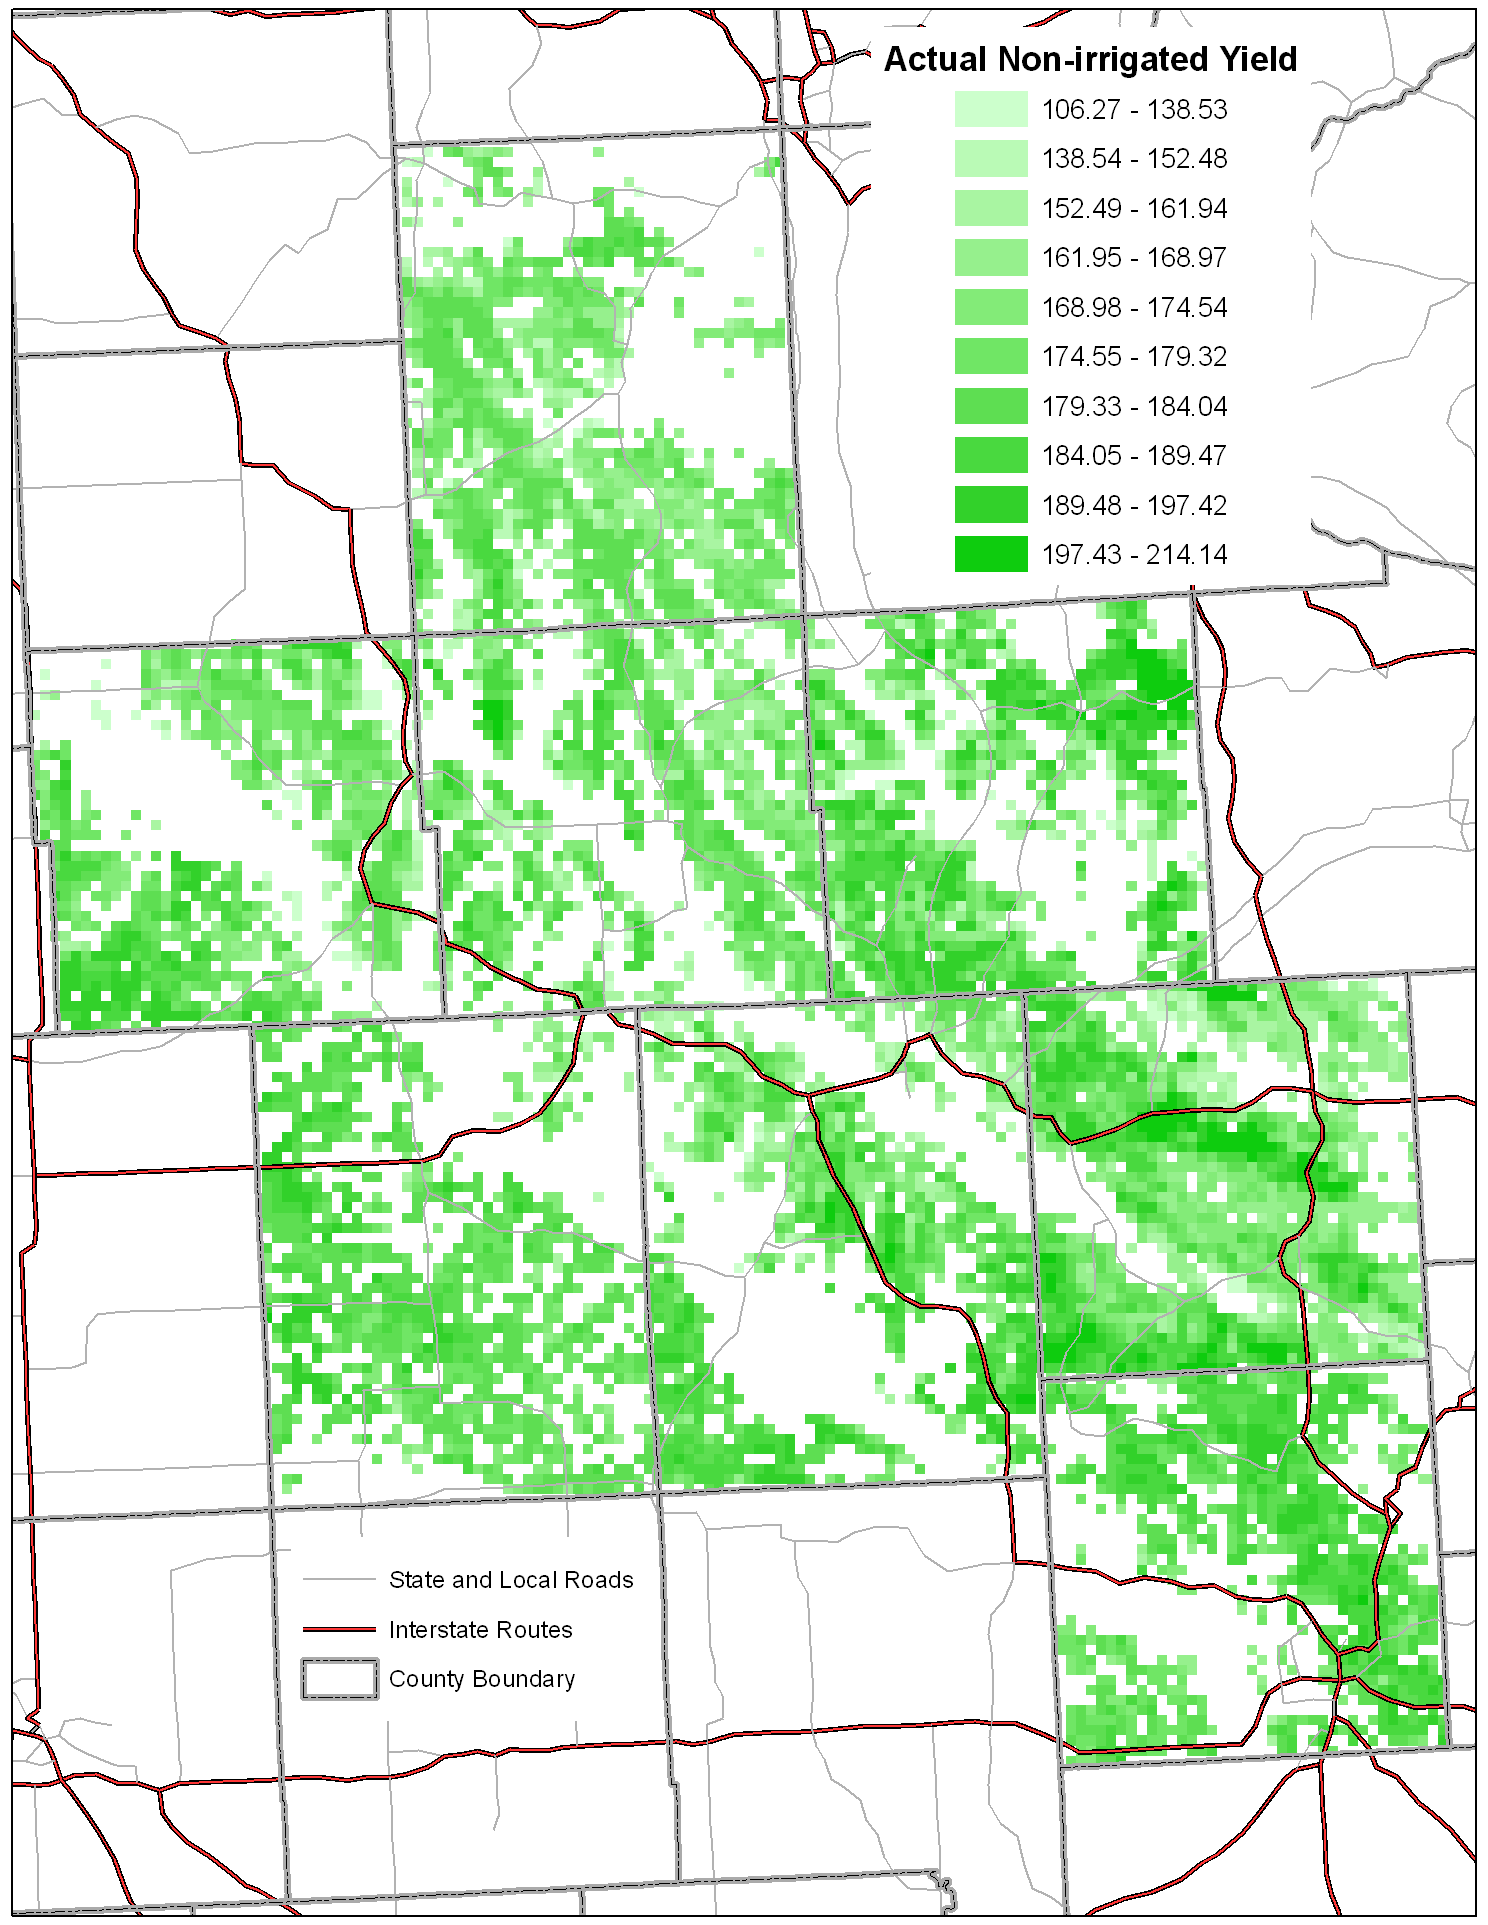
\includegraphics[width=0.45\textwidth]{iowa/farm_costs_nonirr_yield.png}  
  }
  \label{fig:biomass}
  \caption{Pseudo-farm biomass}
\end{figure}

\subsubsection{Forest harvest units}
\label{sec:fhu}




\section{Results}
\label{sec:A1results}

\subsection{Corn Stover}
\label{sec:res_corn}

Eight counties were modeled in this study.  From the total amount of
biomass available from these counties, four refineries were located to
process the biomass.  The refineries were located using a k-means
clustering on the total amount of feedstock, as a method of
approximating equally sized refineries.

Figure~\ref{fig:destination} shows location of the refineries and the
expected destination of the feedstock for each refinery.  This model
is the result of running a network model that includes all roads
within the region, and assigning each pseudo-farm to the refinery
closest to it.  The map shows that despite this more accurate
networking model, feedstocks generally are assigned to the most
geometrically proximate feedstock location.  Also, when refineries
utilize all feedstock, then the feedstock ``sheds'' of the refineries
are necessarily well modeled as circular patterns. 

Figure~\ref{fig:travel} shows a breakdown of the actual travel costs
associated with the individual pseudo-farms within a refinery
region. These costs only include the on-road time costs, and do not
include farmgate, loading, or unloading costs.  As will be seen, this
contributes most to the variation in the supply curves for feedstock
availability.

\begin{figure}[hpt]
  \centering
  \subfigure[Representative Refinery locations and their associated feedstock sheds] {
    \label{fig:destination}
    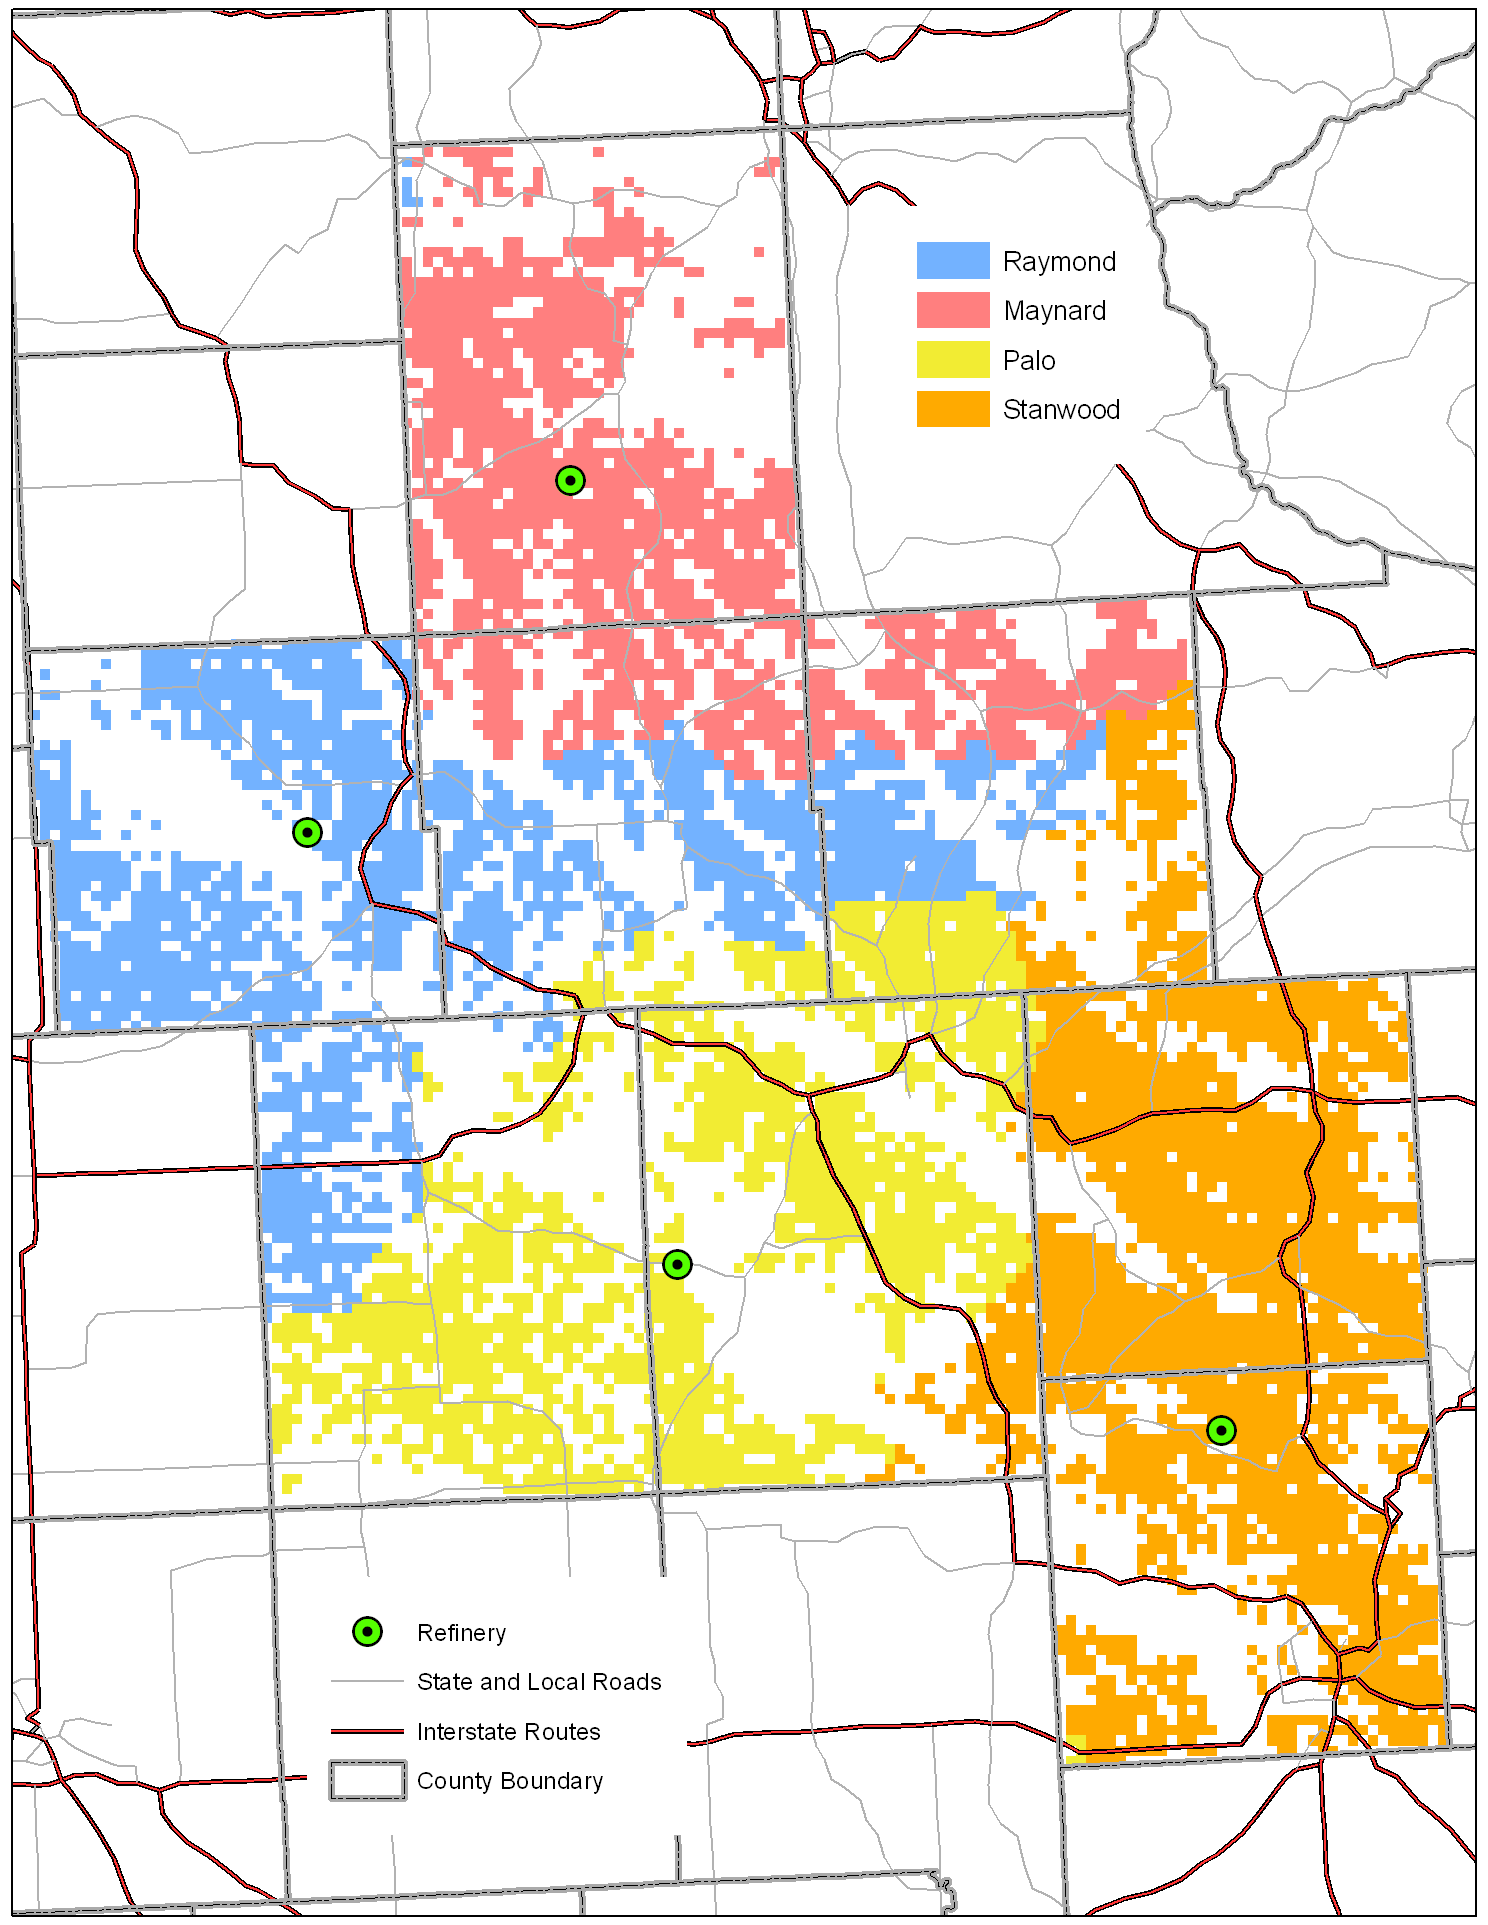
\includegraphics[width=0.45\textwidth]{iowa/farm_costs_destination.png}  
    }
    \subfigure[Travel costs$\cdot bdt^{-1}$ for individual farms] {
      \label{fig:travel}
      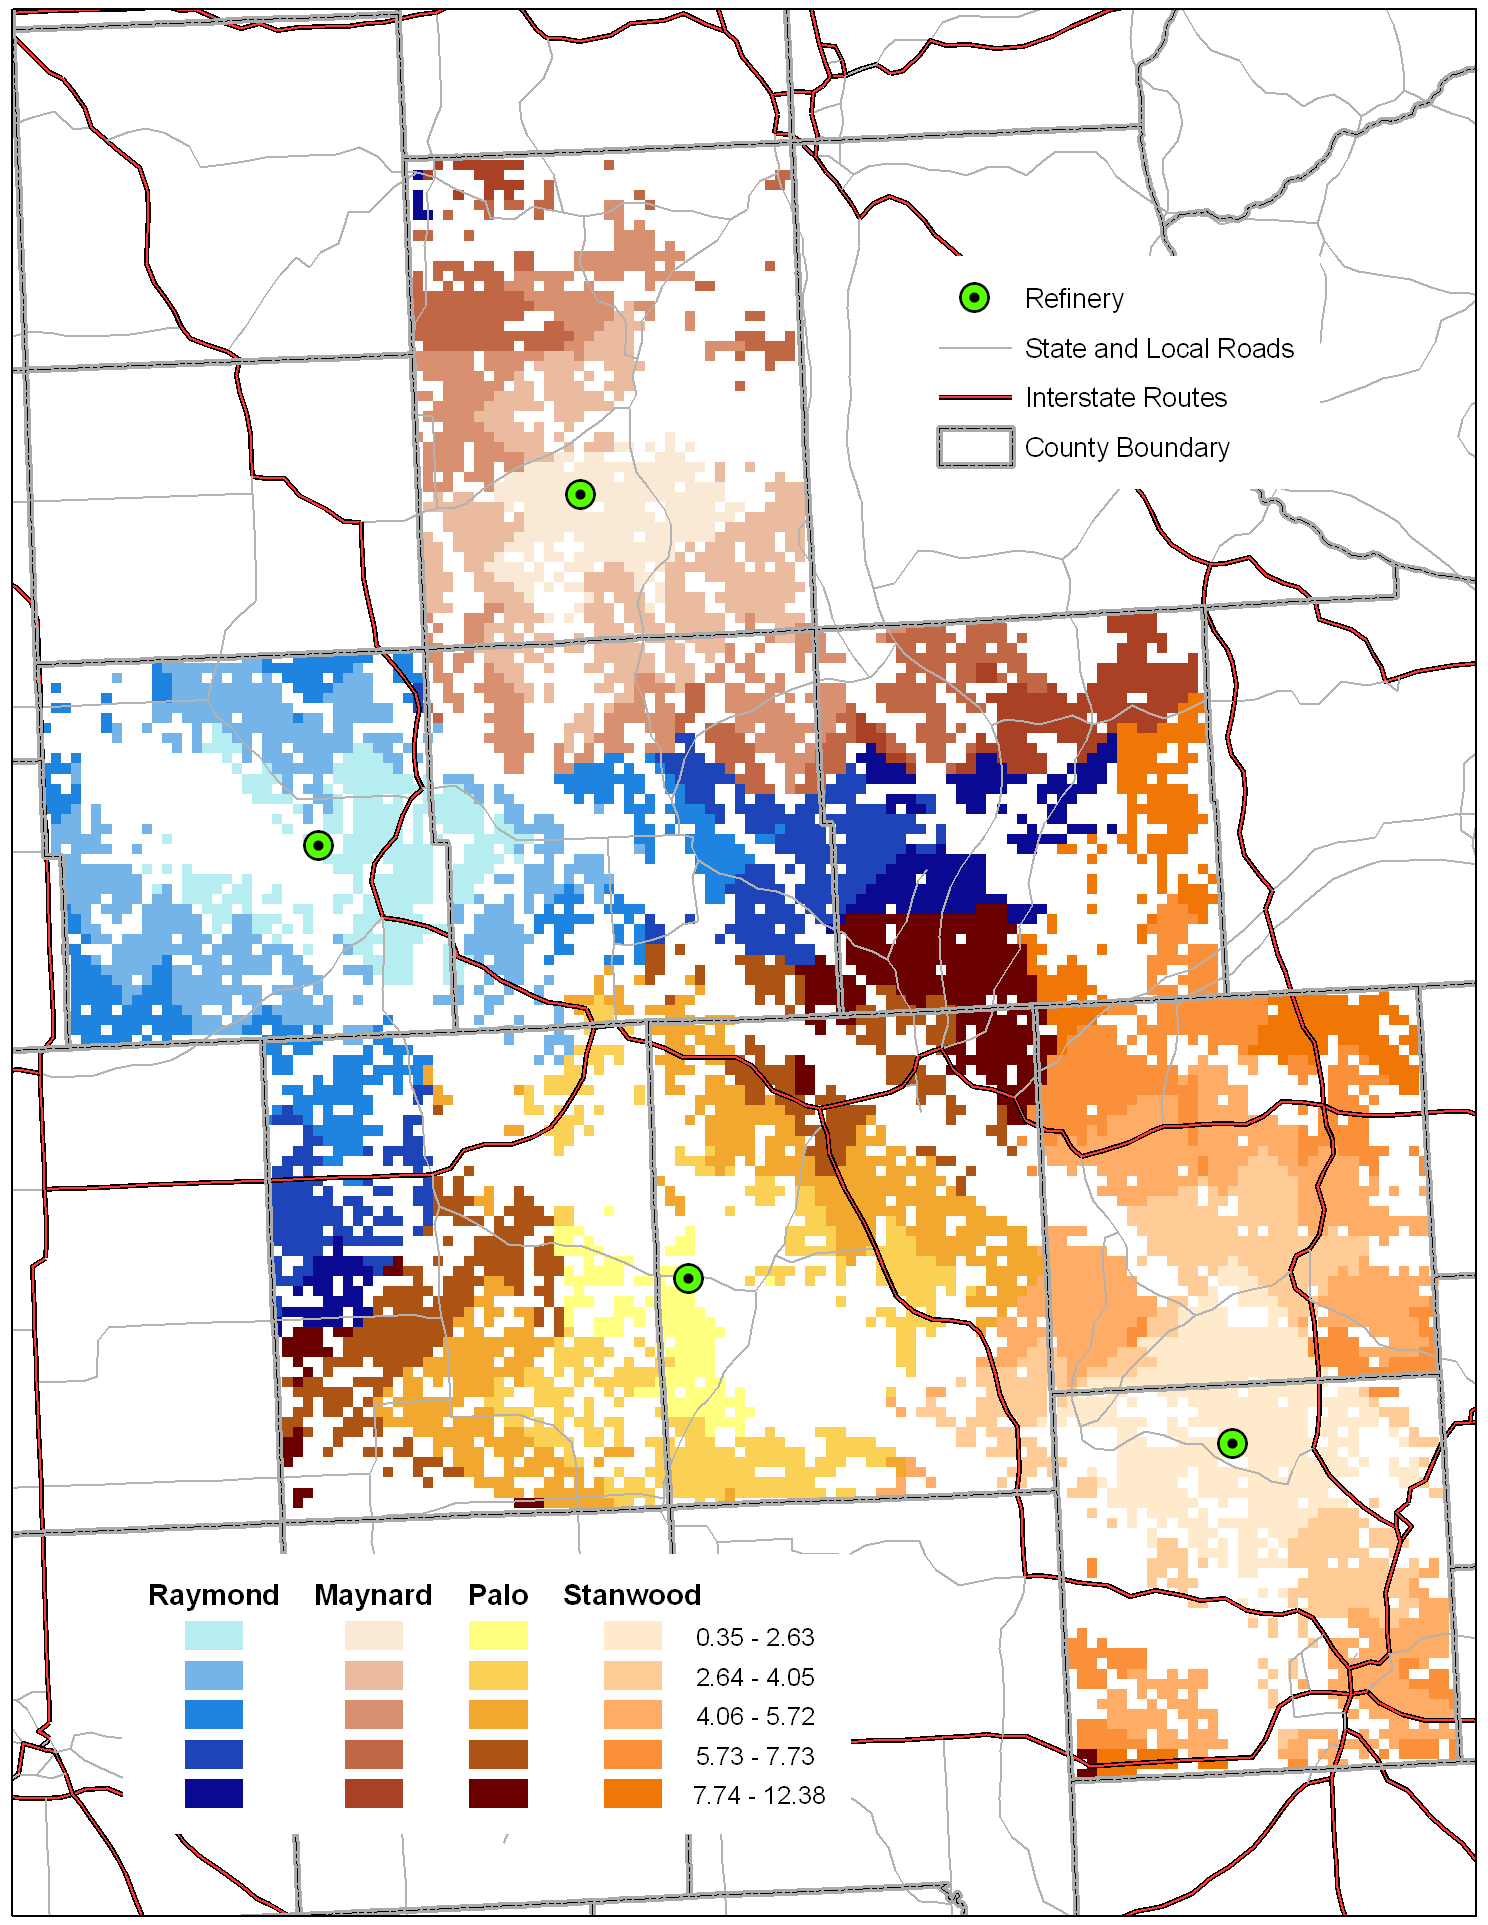
\includegraphics[width=0.45\textwidth]{iowa/farm_costs_travel.png}  
    }
    \caption{Refinery locations and travel costs}
    \label{fig:dest-travel}
\end{figure}


\subsection{Supply curves}

Figure~\ref{fig:supply_curves} shows the individual supply curves for
the 5 refineries in the study region.  The figure shows that despite
the differences in the harvest yields, and transportation
infrastructure, the general shape of the curves are fairly
consistent.

\begin{figure}[hpt]
  \centering
  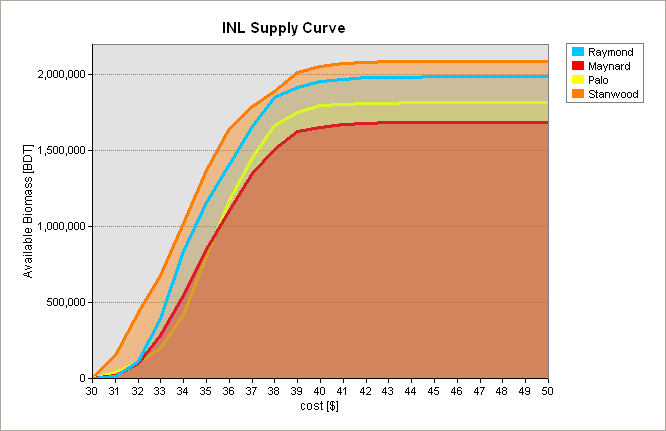
\includegraphics[width=1.0\textwidth]{inlsupplycurve2.png}  
  \caption{Example refinery supply curves for Iowa. }
  \label{fig:supply_curves}
\end{figure}

Figure~\ref{fig:supply_curves_hist} shows this same data as a
histogram, which identifies the range of costs for feedstocks.
Farmgate costs can be affected both by the amount of arable land in
the region as well as by the harvest yields of the biomass.  In
general, however, these vary less than the transportation costs.
Transportation costs are affected by how far the biomass needs to
travel, and in some extent to the speed of the roads being used.
Figures~\ref{fig:farmgate_hist} and~\ref{fig:transportation_hist} show
the various contributions from the farmgate costs and the
transportation costs of the feedstocks

\begin{figure}[hpt]
  \centering
%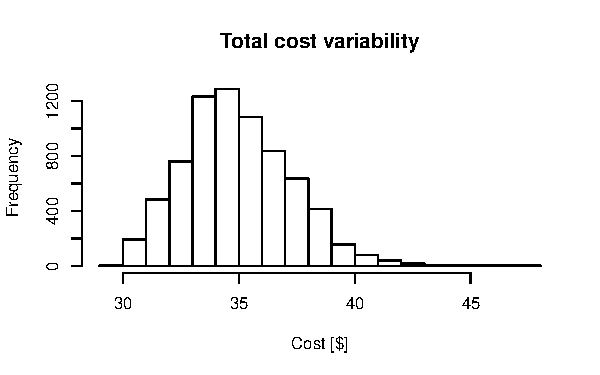
\includegraphics[width=1.0\textwidth]{total.pdf}
  \caption{Total costs $\cdot bdt^{-1}$ of biomass }
  \label{fig:supply_curves_hist}
\end{figure}

\begin{figure}[hpt]
  \centering
%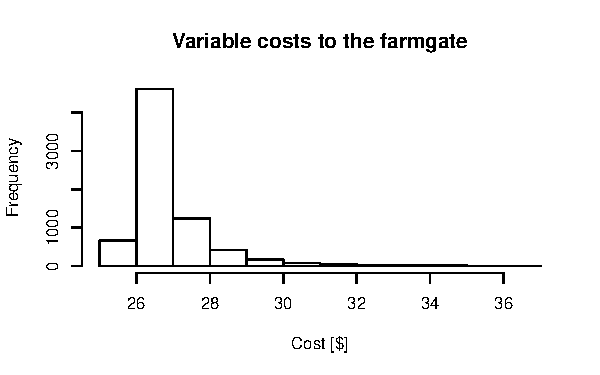
\includegraphics[width=1.0\textwidth]{farmgate.pdf}
  \caption{Farmgate costs $\cdot bdt^{-1}$ }
  \label{fig:farmgate_hist}
\end{figure}

\begin{figure}[hpt]
  \centering
%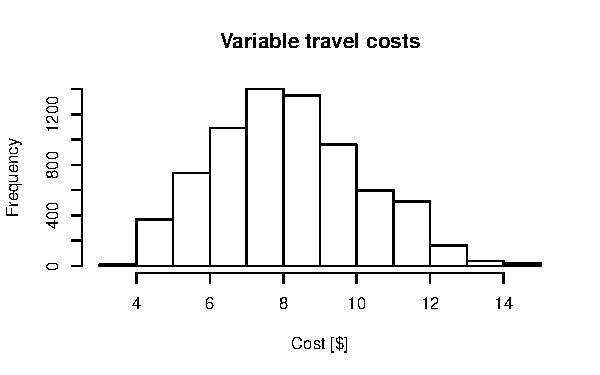
\includegraphics[width=1.0\textwidth]{road_hist.pdf}
  \caption{Transportation costs $\cdot bdt^{-1}$.}
  \label{fig:transportation_hist}
\end{figure}

That transportation is the most variable cost can also be seen in the
utilized feedstock at any given price.  Figure~\ref{fig:supply_curves}
shows that about \%50 of the feedstock is available at \$35.
Figure~\ref{fig:util35} shows the farms that are utilized at this
price.

\begin{figure}[hpt]
  \centering
  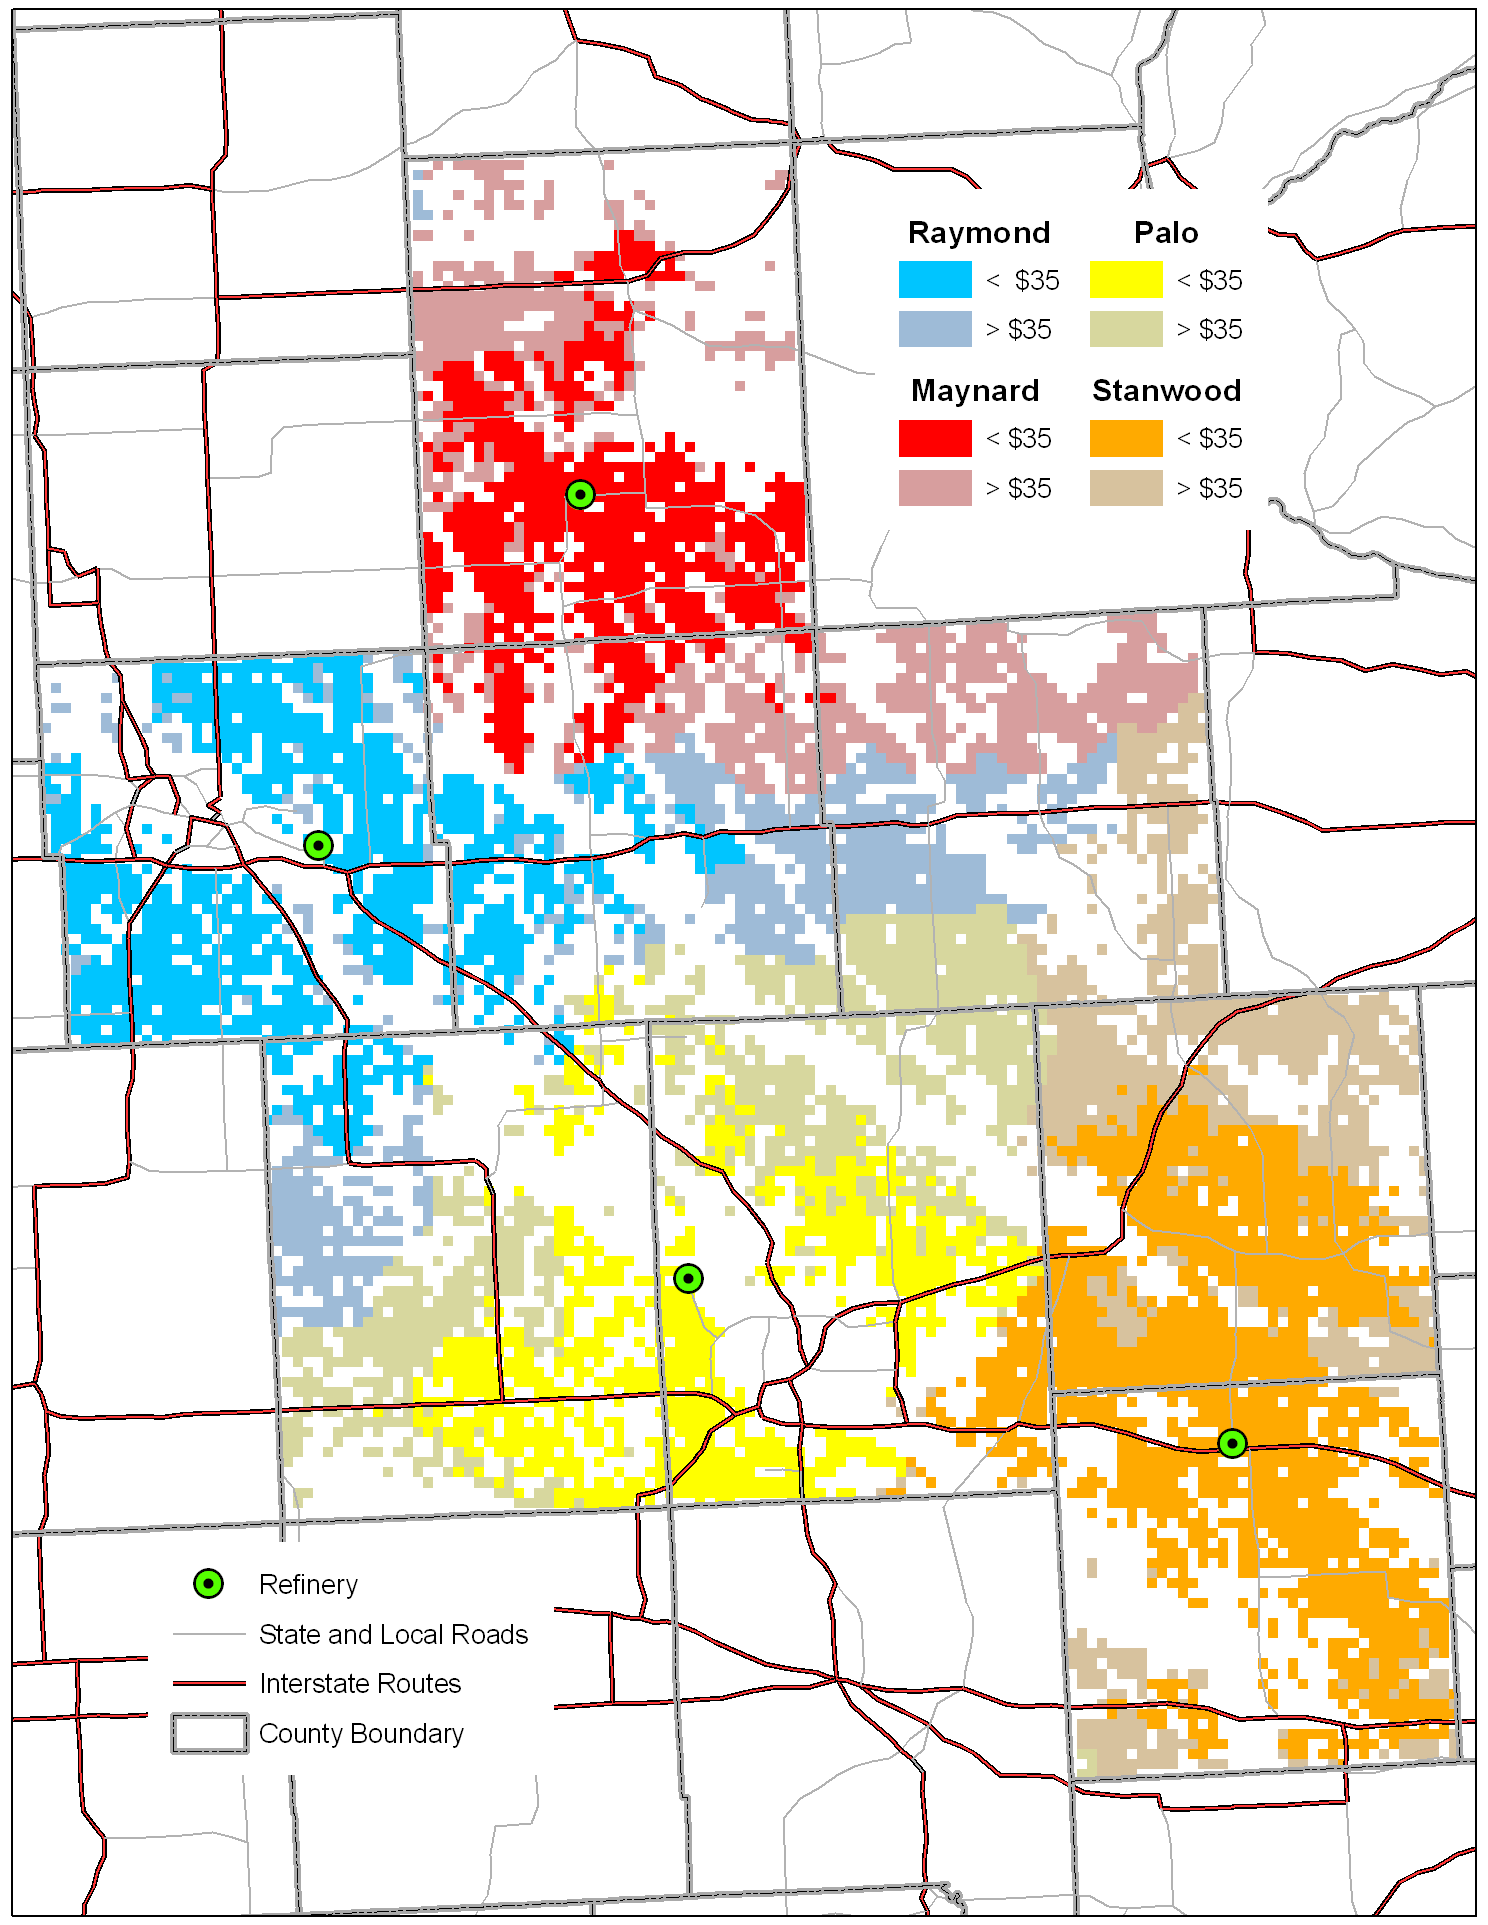
\includegraphics[width=1.0\textwidth]{farm_costs_35dollar_divide.png}  
  \caption{Utilized biomass at $\$35 \cdot bdt^{-1}$. }
  \label{fig:util35}
\end{figure}

\section{Conclusions}
\label{sec:A1conclusions}

\section*{Acronyms}
\begin{acronym}
\acro{FPL}{United States Department of Agriculture Forest Products Lab}
\acro{INL}{Idaho National Laboratory}
\acro{NASS}{National Agricultural Statistics Service}
\end{acronym}

\section{References}
\label{sec:ref}



\bibliography{BandB_qjh_pwt.bib}

\end{document}



